\documentclass[12pt,a4paper]{article}
\usepackage{fontspec}
\usepackage{xeCJK}
\usepackage[expansion=false]{microtype}
\IfFontExistsTF{Latin Modern Roman}{%
  \setmainfont{Latin Modern Roman}%
}{\IfFontExistsTF{Times New Roman}{%
  \setmainfont{Times New Roman}%
}{%
  \setmainfont{Times}%
}}
\IfFontExistsTF{Menlo}{%
  \setmonofont{Menlo}%
}{\IfFontExistsTF{Latin Modern Mono}{%
  \setmonofont{Latin Modern Mono}%
}{}}
% Prefer the project default CJK font, but fall back to common macOS fonts for
% local builds where Noto CJK is not installed.
\IfFontExistsTF{Noto Serif CJK SC}{%
  \setCJKmainfont[ItalicFont={Noto Serif CJK SC}]{Noto Serif CJK SC}%
}{\IfFontExistsTF{PingFang TC}{%
  \setCJKmainfont[ItalicFont={PingFang TC}]{PingFang TC}%
}{\IfFontExistsTF{Hiragino Sans GB}{%
  \setCJKmainfont[ItalicFont={Hiragino Sans GB}]{Hiragino Sans GB}%
}{%
  \setCJKmainfont[ItalicFont={STHeiti}]{STHeiti}%
}}}  
\IfFontExistsTF{Noto Sans Mono CJK SC}{%
  \setCJKmonofont{Noto Sans Mono CJK SC}%
}{\IfFontExistsTF{PingFang TC}{%
  \setCJKmonofont{PingFang TC}%
}{\IfFontExistsTF{Hiragino Sans GB}{%
  \setCJKmonofont{Hiragino Sans GB}%
}{%
  \setCJKmonofont{STHeiti}%
}}}

% Packages
\usepackage{amsmath,amssymb,amsthm}
\usepackage{graphicx}
\usepackage{hyperref}
\usepackage{geometry}
\usepackage{natbib}
\usepackage{booktabs}
\usepackage{tabularx}
% Algorithms not available, using basic formatting
\usepackage{verbatim}
\usepackage{subcaption}
\usepackage{xcolor}
\usepackage{tikz}
\usetikzlibrary{shapes,arrows,positioning}

% Page geometry
\geometry{
  left=2.5cm,
  right=2.5cm,
  top=2.5cm,
  bottom=2.5cm
}

% Theorem environments
\newtheorem{theorem}{定理}[section]
\newtheorem{lemma}[theorem]{引理}
\newtheorem{proposition}[theorem]{命題}
\newtheorem{corollary}[theorem]{推論}

\theoremstyle{definition}
\newtheorem{definition}[theorem]{定義}
\newtheorem{example}[theorem]{範例}

\theoremstyle{remark}
\newtheorem{remark}[theorem]{註記}
\newcommand{\missingfigureplaceholder}{\mbox{}}

% Title information
\title{倫理黎曼猜想：\\
       一個衡量人工智慧道德錯誤增長的數理模型}

\author{李沛宸 \\
        格拉斯哥大學 \\
        1179018@gla.ac.uk}

\date{\today}

\begin{document}

\maketitle

\begin{abstract}
隨著人工智慧系統日益參與道德決策，我們迫切需要嚴謹的框架來理解這些系統何時以及如何出現結構性失敗。本文提出\emph{倫理黎曼猜想}（Ethical Riemann Hypothesis, ERH），這是一個透過與解析數論中質數分布的類比來量化道德判斷系統中錯誤增長模式的數學框架。

我們將「倫理質數」（ethical primes）定義為無法簡化為更簡單案例的基本誤判，並引入$\Pi(x)$作為複雜度級別 $100$ 以下的倫理質數計數函數。透過建立類似於對數積分的基準期望$B(x)$，我們藉由誤差項$E(x) = \Pi(x) - B(x)$來表徵系統性偏差。ERH 指出對於常數$C, \varepsilon > 0$，有$|E(x)| \leq C \cdot x^{1/2 + \varepsilon}$，這表明「健康」判斷系統中的錯誤最多以次線性方式增長。

透過比較偏見、隨機、保守和激進等四種判斷策略的計算模擬（基於 2000 個行動的實驗），我們發現不同系統表現出顯著不同的錯誤增長模式：激進與偏見判斷者顯示快速下降的誤差項（$\alpha < -0.4$），而隨機與保守判斷者則呈現較為平坦的模式（$\alpha \approx -0.1$）。值得注意的是，所有判斷者雖在誤差增長模式上落在 ERH 式上界之內，但保守判斷者的高錯誤率（61.1\%）提醒我們，長尾誤差受控並不等於整體判斷品質良好。

此框架為評估 AI 道德判斷系統與識別結構性偏見提供了定量診斷視角，並可作為機器學習公平性、演算法問責制以及自動化道德推理中的補充審計工具。

\textbf{關鍵詞：}倫理黎曼猜想、人工智慧倫理、道德判斷、錯誤分析、AI 公平性、質數理論、結構性偏見
\end{abstract}

% ============================================
% 第一節：緒論
% ============================================
\section{緒論}
\label{sec:introduction}

\subsection{研究動機}

道德判斷的挑戰對人類社會和人工智慧系統都至關重要。隨著 AI 日益參與影響人類福祉的決策---從刑事司法和醫療診斷到資源分配和內容審核---我們需要嚴謹的框架來理解這些系統何時以及如何失敗 \citep{jobin2019,floridi2018}。

傳統的 AI 倫理方法通常關注：
\begin{itemize}
    \item \textbf{基於規則的框架}：定義明確的道德規則（例如，阿西莫夫的機器人三定律）
    \item \textbf{結果主義}：優化結果（例如，功利主義計算）
    \item \textbf{公平性指標}：測量統計均等、機會均等、校準 \citep{hardt2016,dwork2012}
\end{itemize}

雖然有價值，但這些方法通常分析個別案例或聚合統計。它們對誤判的\emph{結構性模式}提供有限的洞察：錯誤如何隨著問題複雜度增加而累積？是否存在會透過系統級聯的基本誤判？判斷系統何時變得系統性地不可靠？

\subsection{與質數的類比}

我們提出一個意想不到的類比：\emph{關鍵道德誤判的分布類似於質數的分布} \citep{riemann1859,edwards1974}。

在數論中：
\begin{itemize}
    \item 質數是算術的「原子」---不可約的建構塊
    \item 它們的分布看似不規則但遵循深層模式
    \item 黎曼猜想表徵了計數質數時的誤差
    \item 這個誤差項編碼了關於數論結構的深刻資訊
\end{itemize}

在道德判斷中：
\begin{itemize}
    \item 某些誤判是「倫理質數」---無法簡化為更簡單案例的基本錯誤
    \item 它們在複雜度級別上的分布看似不規則但可能遵循模式
    \item 「倫理黎曼猜想」可以表徵計數這些質數時的誤差
    \item 這個誤差項編碼了關於判斷系統結構健康狀況的資訊
\end{itemize}

\subsection{研究貢獻}

本文做出以下貢獻：

\begin{enumerate}
    \item \textbf{數學形式化}：我們在嚴謹的數學框架中定義行動空間、真實道德值、判斷函數和倫理質數（第\ref{sec:formalization}節）。
    
    \item \textbf{倫理黎曼猜想}：我們精確地陳述 ERH 並解釋其對判斷系統品質的意義（第\ref{sec:erh}節）。
    
    \item \textbf{計算框架}：我們開發模擬工具來實證測試不同判斷系統的 ERH（第\ref{sec:framework}節）。
    
    \item \textbf{實證結果}：我們展示偏見、隨機、保守和激進的判斷者具有不同的錯誤模式，且落在 ERH 式上界之內並不保證整體判斷品質（第\ref{sec:results}節）。
    
    \item \textbf{哲學意涵}：我們將 ERH 與古典道德哲學聯繫起來，並討論其對 AI 倫理的意涵（第\ref{sec:philosophy}節）。
    
    \item \textbf{AI 倫理應用}：我們討論 ERH 如何作為 AI 系統的結構診斷約束，並說明其必要但非充分的定位（第\ref{sec:implications}節）。
\end{enumerate}

\subsection{論文組織}

本文其餘部分組織如下。第\ref{sec:related}節回顧相關研究和理論基礎。第\ref{sec:formalization}節發展數學形式化。第\ref{sec:erh}節陳述倫理黎曼猜想及其變體。第\ref{sec:framework}節描述我們的計算框架。第\ref{sec:results}節呈現實驗結果。第\ref{sec:philosophy}節討論哲學意涵。第\ref{sec:implications}節討論對 AI 倫理的應用。第\ref{sec:conclusion}節總結並概述未來工作。

% ============================================
% 第二節：相關研究與理論基礎
% ============================================
\section{相關研究與理論基礎}
\label{sec:related}

\subsection{AI 判斷錯誤與倫理風險}

關於 AI 倫理的文獻廣泛記錄了演算法系統中各種形式的偏見和不公平 \citep{mehrabi2021,barocas2016,oneil2016}。然而，大多數方法關注公平性的統計測量（例如，人口統計均等、均等化機會）或個別案例分析，而不是錯誤累積的結構性模式。

\citet{binns2018} 認為機器學習中的公平性應該從政治哲學中汲取，特別是分配正義理論。\citet{selbst2019} 強調公平性必須在社會技術系統中理解，而不是作為孤立的演算法屬性。雖然這些工作提供了重要的理論基礎，但它們缺乏測量結構性退化的定量框架。

\subsection{數學模型在 AI 倫理中的應用}

幾位研究人員已將數學形式化應用於倫理問題。\citet{dwork2012} 透過意識引入了公平性的正式定義，使用度量空間來量化相似性。然而，這些方法關注靜態屬性而不是動態錯誤增長模式。在形式語意與意向邏輯脈絡中，Cohen 與 Levesque 則提出將意向視為具承諾的選擇的經典模型 \citep{cohen1990}，為後續的義務／意向邏輯研究奠定基礎。

\subsection{哲學中的隱喻模型}

數學隱喻在哲學中的使用有著豐富的歷史。控制論隱喻已應用於倫理學 \citep{floridi2018}，博弈論已用於建模道德困境。我們的方法透過使用解析數論作為理解道德判斷系統的透鏡來擴展這一傳統。

\subsection{數論中的黎曼猜想}

經典的黎曼猜想由 \citet{riemann1859} 提出，涉及黎曼 zeta 函數 $\zeta(s)$ 的零點分布。\citet{montgomery1973} 顯示零點的配對相關遵循特定模式，表明質數分布中的深層結構。\citet{granville2007} 進一步發展了字符和與質數分布之間的聯繫。

雖然黎曼猜想仍未得到證明，但它對質數分布的意涵是深遠的。我們將此框架適應於倫理質數，認識到類比是啟發性的但可能具有啟發性。

\subsection{缺口分析}

當前 AI 倫理方法存在幾個限制：
\begin{itemize}
    \item \textbf{缺乏結構性分析}：大多數方法分析個別案例或聚合統計，錯過了錯誤累積的模式
    \item \textbf{沒有複雜度感知指標}：現有的公平性指標不考慮錯誤如何隨問題複雜度擴展
    \item \textbf{形式化不足}：很少有框架為倫理錯誤模式提供嚴謹的數學模型
    \item \textbf{缺少預測標準}：沒有定量標準來判斷判斷系統何時變得系統性地不可靠
\end{itemize}

我們的 ERH 框架透過提供結構性、複雜度感知、形式嚴謹且可診斷的倫理錯誤模式模型來解決這些缺口。

\begin{table}[htbp]
\centering
\caption{現有方法與 ERH 框架的比較}
\label{tab:comparison}
\begin{tabular}{lcc}
\toprule
\textbf{特徵} & \textbf{現有方法} & \textbf{ERH 框架} \\
\midrule
分析層級 & 個別/聚合 & 結構性 \\
複雜度感知 & 否 & 是 \\
數學嚴謹性 & 有限 & 高 \\
預測能力 & 低 & 高 \\
錯誤增長模型 & 無 & 次線性界限 \\
\bottomrule
\end{tabular}
\end{table}

% ============================================
% 第三節：模型建構
% ============================================
\section{模型建構}
\label{sec:formalization}

\subsection{行動空間}

\begin{definition}[行動空間]
\emph{行動空間}是一個有限集合 $\mathcal{A} = \{a_1, a_2, \ldots, a_N\}$，其中每個行動 $a_i$ 具有以下屬性：
\begin{itemize}
    \item \textbf{複雜度} $c(a) \in \mathbb{N}$：表示決策複雜度的正整數（資訊需求、利益相關者數量、不確定性等）
    \item \textbf{真實道德值} $V(a) \in \mathbb{R}$：「真實情況」的倫理評估，通常歸一化為 $[-1, 1]$，其中 $-1$ 是最大有害，$0$ 是中性的，$+1$ 是最大有益
    \item \textbf{重要性權重} $w(a) \in \mathbb{R}^+$：行動的重要性（受影響的人數、後果的嚴重程度等）
\end{itemize}
\end{definition}

\begin{remark}
真實道德值 $V(a)$ 代表理想化的「上帝視角」或完美道德推理者之間的共識。在實踐中，這是無法獲得的，必須近似。在我們的模擬中，我們明確地將 $V(a)$ 定義為真實情況。
\end{remark}

\subsection{判斷系統}

\begin{definition}[判斷系統]
\emph{判斷系統} $\mathcal{J}$ 是一個為每個行動分配道德評估的函數：
\[
\mathcal{J}: \mathcal{A} \to \mathbb{R}
\]
我們將 $J(a) = \mathcal{J}(a)$ 表示為行動 $a$ 的判斷。
\end{definition}

\begin{definition}[判斷誤差]
判斷 $\mathcal{J}$ 對行動 $a$ 的\emph{誤差}為：
\[
\Delta(a) = J(a) - V(a)
\]
如果對於某個閾值 $\tau > 0$，有 $|\Delta(a)| > \tau$，則判斷被視為\emph{錯誤}。
\end{definition}

我們定義二元錯誤指標：
\[
M(a) = \begin{cases}
1 & \text{如果 } |\Delta(a)| > \tau \\
0 & \text{否則}
\end{cases}
\]

\subsection{倫理質數}

\begin{definition}[倫理質數]
行動 $a \in \mathcal{A}$ 是\emph{倫理質數}，如果：
\begin{enumerate}
    \item $M(a) = 1$（它被誤判）
    \item $w(a)$ 很大（高重要性，通常在頂部分位數）
    \item $a$ 是「結構性基本」：糾正此錯誤將顯著減少整體誤判
\end{enumerate}
\end{definition}

讓 $\mathcal{P} \subseteq \mathcal{A}$ 表示倫理質數的集合。在實踐中，我們透過重要性分位數和複雜度範圍過濾誤判行動來選擇 $\mathcal{P}$。

\begin{proposition}[倫理質數集合的穩定性]
\label{prop:prime_stability}
給定行動空間 $\mathcal{A}$ 和判斷系統 $\mathcal{J}$，設重要性閾值為 $w_0$，則倫理質數集合 $\mathcal{P}$ 滿足：
\[
|\mathcal{P}| \leq \min\left(|\{a \in \mathcal{A} : M(a) = 1\}|, |\{a \in \mathcal{A} : w(a) \geq w_0\}|\right)
\]
進一步，若判斷系統滿足一致誤差界 $|\Delta(a)| \leq \delta$ 對於所有 $a \in \mathcal{A}$，且誤差閾值 $\tau > \delta$，則 $\mathcal{P} = \emptyset$。相反，若存在某個複雜度級別 $c_0$ 使得對於所有 $c(a) \geq c_0$ 的行動，誤差 $|\Delta(a)| > \tau$ 且 $w(a) \geq w_0$ 的概率為 $p > 0$，則期望倫理質數數量至少為 $p \cdot |\{a \in \mathcal{A} : c(a) \geq c_0, w(a) \geq w_0\}|$。
\end{proposition}

\begin{proof}[證明概要]
第一個不等式直接來自倫理質數的定義：它必須既是錯誤（$M(a) = 1$）又具有高重要性（$w(a) \geq w_0$）。若一致誤差界成立，則對於所有行動 $|\Delta(a)| \leq \delta < \tau$，因此 $M(a) = 0$ 對於所有 $a$，導致 $\mathcal{P} = \emptyset$。最後的期望值來自概率論的基本性質：若每個滿足條件的行動以概率 $p$ 成為倫理質數，則期望數量為概率與數量的乘積。
\end{proof}

\subsection{判斷者類型的理論區分}

不同類型的判斷系統在誤差結構上表現出不同的理論特徵。我們可以對每種類型建立誤差上界與期望行為：

\begin{proposition}[偏見判斷者的誤差結構]
\label{prop:biased_error}
對於偏見判斷者，設偏見函數 $b(c)$ 單調遞增且 $b(0) = 0$，雜訊方差 $\sigma^2$，則期望誤差為：
\[
\mathbb{E}[|\Delta(a)|] \geq |b(c(a))| - \sigma \sqrt{\frac{2}{\pi}}
\]
若 $b(c) = b_0 \cdot c^\beta$ 對於某些 $b_0 > 0, \beta > 0$，則誤差隨複雜度增長，倫理質數在 $c(a)$ 較大的範圍內更容易出現。
\end{proposition}

\begin{proposition}[隨機判斷者的誤差結構]
\label{prop:noisy_error}
對於隨機判斷者，設雜訊方差 $\sigma^2(c)$ 可能隨複雜度變化，則誤差的方差為：
\[
\text{Var}[\Delta(a)] = \sigma^2(c(a))
\]
若 $\sigma(c) = \sigma_0 \cdot c^\gamma$ 對於 $\sigma_0 > 0, \gamma \geq 0$，則高複雜度案例的誤差變異性更大。當 $\gamma > 0$ 時，誤差增長指數 $\alpha$ 傾向於接近 $0$，因為誤差主要受隨機性主導而非系統性模式。
\end{proposition}

\begin{proposition}[保守判斷者的誤差結構]
\label{prop:conservative_error}
對於保守判斷者，設收縮因子 $\lambda(c) \in [0,1]$ 隨複雜度單調遞增，則期望誤差為：
\[
\mathbb{E}[|\Delta(a)|] \approx |V(a)| \cdot \lambda(c(a))
\]
保守策略導致所有判斷向中性收縮，因此低複雜度案例（$|V(a)|$ 接近 $1$）可能出現較大誤差，而高複雜度模糊案例（$|V(a)| \approx 0$）誤差較小。這解釋了保守判斷者為何具有最高的錯誤率但接近零的誤差增長指數。
\end{proposition}

\begin{proposition}[激進判斷者的誤差結構]
\label{prop:radical_error}
對於激進判斷者，設放大因子 $\alpha > 1$，則誤差為：
\[
\Delta(a) = (\alpha - 1) \cdot V(a) + \mathcal{N}(0, \sigma^2)
\]
當 $|V(a)|$ 較大時，放大導致顯著誤差；當 $|V(a)| \approx 0$ 時，誤差主要由雜訊主導。因此激進判斷者在低複雜度清晰案例中表現較差，但在高複雜度模糊案例中可能提供更清晰的判別信號，導致誤差隨複雜度增加而下降。
\end{proposition}

\subsection{計數函數}

\begin{definition}[倫理質數計數函數]
定義 $\Pi(x)$ 為複雜度最多為 $x$ 的倫理質數數量：
\[
\Pi(x) = \#\{p \in \mathcal{P} : c(p) \leq x\}
\]
\end{definition}

\begin{definition}[基準函數]
\emph{基準函數} $B(x)$ 表示在平滑模型下，複雜度最多為 $x$ 的倫理質數的預期數量。我們考慮幾種形式：
\begin{enumerate}
    \item \textbf{線性}：對於某個 $\alpha > 0$，$B(x) = \alpha x$
    \item \textbf{質數定理類比}：對於某個 $\beta > 0$，$B(x) = \beta \frac{x}{\log x}$，直接類比於質數定理
    \item \textbf{對數積分}：$B(x) = \beta \cdot \text{Li}(x)$，其中 $\text{Li}(x) = \int_2^x \frac{dt}{\log t}$
    \item \textbf{冪律}：對於參數 $\gamma, \delta > 0$，$B(x) = \gamma x^\delta$
\end{enumerate}
\end{definition}

\begin{definition}[誤差項]
\emph{誤差項}為：
\[
E(x) = \Pi(x) - B(x)
\]
這測量了倫理質數的實際分布與基準期望的偏差。
\end{definition}

\subsection{範例：計算 \texorpdfstring{$\Pi(x)$}{Pi(x)}}

考慮一個簡單範例，包含三個行動：
\begin{itemize}
    \item $a_1$：$c(a_1) = 5$，$V(a_1) = 0.8$，$w(a_1) = 10$，$|\Delta(a_1)| = 0.4$（錯誤）
    \item $a_2$：$c(a_2) = 15$，$V(a_2) = -0.6$，$w(a_2) = 8$，$|\Delta(a_2)| = 0.5$（錯誤）
    \item $a_3$：$c(a_3) = 20$，$V(a_3) = 0.3$，$w(a_3) = 12$，$|\Delta(a_3)| = 0.2$（非錯誤）
\end{itemize}

如果 $\tau = 0.3$ 且我們選擇倫理質數作為錯誤中重要性前 50\%，則 $\mathcal{P} = \{a_1, a_2\}$（兩者都是錯誤，且 $a_1$ 具有最高重要性）。那麼：
\begin{align*}
\Pi(10) &= 1 \quad \text{（只有 $a_1$ 的 $c \leq 10$）} \\
\Pi(15) &= 2 \quad \text{（$a_1$ 和 $a_2$ 的 $c \leq 15$）} \\
\Pi(20) &= 2 \quad \text{（兩者的 $c \leq 20$）}
\end{align*}

% ============================================
% 第四節：倫理黎曼猜想
% ============================================
\section{倫理黎曼猜想}
\label{sec:erh}

\subsection{ERH 的陳述}

\begin{theorem}[倫理黎曼猜想（ERH）]
\label{thm:erh}
讓 $\mathcal{J}$ 為判斷系統，並讓 $E(x) = \Pi(x) - B(x)$ 為其倫理質數分布的誤差項。如果存在常數 $C, \varepsilon > 0$，使得對於複雜度範圍內的所有 $x$：
\[
|E(x)| \leq C \cdot x^{1/2 + \varepsilon}
\]
則判斷系統滿足\emph{倫理黎曼猜想}。此界限 $|E(x)| \leq C \cdot x^{1/2 + \varepsilon}$ 稱為\emph{ERH 式界限}。
\end{theorem}

\begin{remark}[ERH 作為必要但非充分條件]
\label{rem:erh_necessary}
ERH 式界限 $|E(x)| \leq C \cdot x^{1/2 + \varepsilon}$ 提供了判斷系統結構健康的\emph{必要條件}：它確保誤差增長保持次線性且有界。然而，僅滿足此界限並\emph{不足以}保證系統在道德上可接受。判斷系統還必須維持低整體錯誤率並避免系統性偏見。如我們的實驗結果所示（第~\ref{sec:results}節），系統可能滿足 ERH 式界限但仍表現出不可接受的高錯誤率（例如錯誤率為 61.1\% 的保守判斷者）。因此，ERH 式界限應與其他指標（如整體準確度、公平性測量、領域特定品質標準）一起評估。
\end{remark}

\subsection{直觀解釋}

ERH 指出，預測關鍵誤判時的累積誤差最多以 $\sqrt{x}$ 的速度增長（最多到一個小因子 $x^\varepsilon$）。這是一個\emph{次線性}增長率，意味著：

\begin{itemize}
    \item 隨著問題複雜度增加，判斷系統不會失控
    \item 錯誤緩慢且可預測地累積
    \item 系統在各種規模下保持結構完整性
\end{itemize}

\subsection{與經典黎曼猜想的比較}

\begin{table}[htbp]
\centering
\caption{經典 RH 與 ERH 的類比}
\label{tab:analogy}
\begin{tabular}{ll}
\toprule
\textbf{數論} & \textbf{倫理判斷} \\
\midrule
自然數 $n$ & 行動複雜度 $c$ \\
質數 $p$ & 倫理質數（關鍵誤判） \\
$\pi(x)$（質數計數） & $\Pi(x)$（倫理質數計數） \\
$\text{Li}(x) \sim \frac{x}{\log x}$ & $B(x) \sim \frac{x}{\log x}$ \\
$E(x) = \pi(x) - \text{Li}(x)$ & $E(x) = \Pi(x) - B(x)$ \\
RH: $|E(x)| = O(x^{1/2} \log x)$ & ERH: $|E(x)| = O(x^{1/2 + \varepsilon})$ \\
$\zeta(s)$ 黎曼 zeta 函數 & $\zeta_E(s)$ 倫理 zeta 函數 \\
$\zeta(s)$ 的零點 & $\zeta_E(s)$ 的零點 \\
\bottomrule
\end{tabular}
\end{table}

\subsection{倫理 Zeta 函數}

我們可以透過生成函數定義「倫理 zeta 函數」：

\begin{definition}[倫理 Zeta 函數]
讓 $m(n)$ 為複雜度級別 $n$ 的倫理質數數量（或加權計數）。定義：
\[
\zeta_E(s) = \sum_{n=1}^{N} \frac{m(n)}{n^s}
\]
對於 $s \in \mathbb{C}$，其中 $\text{Re}(s) > 1$。
\end{definition}

\subsection{倫理 Zeta 函數的解析性質}

雖然倫理 zeta 函數 $\zeta_E(s)$ 是有限和（與經典黎曼 zeta 函數的無窮級數不同），我們仍可以分析其基本解析性質，並建立與誤差項 $E(x)$ 的啟發式關聯。

\begin{proposition}[收斂域與解析性]
\label{prop:zeta_convergence}
倫理 zeta 函數 $\zeta_E(s)$ 在所有 $s \in \mathbb{C}$ 上定義（因為是有限和），但它在 $\text{Re}(s) > 1$ 區域內表現出類似於經典 zeta 函數的結構特性。若 $m(n) = O(n^\delta)$ 對於某個 $\delta < 1$，則在 $\text{Re}(s) > \delta + 1$ 的區域內，$\zeta_E(s)$ 的增長主要由低複雜度項主導。
\end{proposition}

\begin{proposition}[零點分布與誤差項的啟發式關聯]
\label{prop:zeros_error_heuristic}
（啟發性、非嚴格）若倫理 zeta 函數 $\zeta_E(s)$ 的零點集中在某條臨界線附近（例如 $\text{Re}(s) = \sigma_0$），則誤差項 $E(x)$ 的增長率可能與 $\sigma_0$ 相關：
\[
|E(x)| \sim x^{\sigma_0} \quad \text{(啟發性)}
\]
具體而言，若零點集中在 $\text{Re}(s) = 1/2$ 附近，則可能表明 $|E(x)| = O(x^{1/2 + \varepsilon})$，這與 ERH 的預測一致。這是一個啟發式類比，而非嚴格定理，因為經典 zeta 函數的零點與質數分布誤差項的關聯涉及複雜的解析數論技術（如 Perron 公式與 Mellin 變換），而我們的有限和版本不具備相同程度的理論結構。
\end{proposition}

\begin{remark}[類比的啟發價值與限制]
倫理 zeta 函數與經典黎曼 zeta 函數的類比具有啟發價值，但存在重要差異：
\begin{itemize}
    \item \textbf{有限性}：$\zeta_E(s)$ 是有限和，因此沒有解析延拓、函數方程或臨界帶的概念，這些是經典 zeta 函數的關鍵特徵。
    \item \textbf{結構差異}：倫理質數的分布可能不具備質數分布的深層數論結構（如算術級數中的質數定理）。
    \item \textbf{啟發性價值}：儘管如此，零點分析仍可能揭示誤差分布中的週期性模式，頻譜分析（對應於離散傅立葉變換）可識別複雜度級別之間的相關性。
\end{itemize}
\end{remark}

$\zeta_E(s)$ 在複平面中的零點分布編碼了倫理質數分布的「週期性」或「規律性」資訊。如果零點在臨界線附近聚集（類似於黎曼 zeta 的 $\text{Re}(s) = 1/2$），這表明判斷錯誤中的深層結構規律性。然而，我們必須認識到這是一個啟發式類比，而非嚴格的數論對應關係。

% ============================================
% 第五節：模擬設計與實驗方法
% ============================================
\section{模擬設計與實驗方法}
\label{sec:framework}

\subsection{行動空間生成}

我們從以下分布生成複雜度樣本的行動：
\begin{itemize}
    \item \textbf{均勻分布}：$c(a) \sim \text{Uniform}(1, C_{\max})$
    \item \textbf{Zipf 分布}：$c(a) \sim \text{Zipf}(\alpha)$（更現實，許多簡單案例，少數複雜）
    \item \textbf{冪律}：$c(a) \sim x^{-\gamma}$
\end{itemize}

真實道德值 $V(a)$ 以\emph{複雜度依賴的模糊性}生成：
\begin{itemize}
    \item 低複雜度：清晰的值（接近 $\pm 1$）
    \item 高複雜度：模糊的值（接近 $0$）
\end{itemize}

這反映了簡單道德案例通常是明確的，而複雜案例涉及多個競爭考慮的直覺。

\subsection{判斷系統模型}

我們實現五種典型判斷者：

\begin{enumerate}
    \item \textbf{偏見判斷者}：系統性偏見 $b(c)$ 隨複雜度增加：
    \[
    J(a) = V(a) + b_0 \cdot f(c(a)) + \mathcal{N}(0, \sigma^2)
    \]
    其中 $f(c)$ 是單調遞增的。
    
    \item \textbf{隨機判斷者}：高隨機雜訊：
    \[
    J(a) = V(a) + \mathcal{N}(0, \sigma^2(c))
    \]
    其中雜訊隨複雜度擴展。
    
    \item \textbf{保守判斷者}：向中性收縮：
    \[
    J(a) = (1-\lambda(c)) V(a) + \mathcal{N}(0, \sigma^2)
    \]
    其中 $\lambda(c) \in [0,1]$ 隨複雜度增加。
    
    \item \textbf{激進判斷者}：放大極端：
    \[
    J(a) = \alpha \cdot V(a) + \mathcal{N}(0, \sigma^2)
    \]
    其中 $\alpha > 1$。
    
    \item \textbf{量子判斷者}：基於疊加態的量子測量判斷。令 $\theta = c(a)/100 \cdot \pi$；對 $|0\rangle$ 施加 Rx$(\theta)$ 旋轉。測量得 $J(a) = 2|\alpha|^2 - 1 \in [-1, 1]$，其中 $|\alpha|^2$ 為測得「倫理」（$|0\rangle$）之機率。可用 qiskit-aer 或 NumPy 後備以確保可重現性。
\end{enumerate}

\subsection{分析流程}

對於每個判斷系統：
\begin{enumerate}
    \item 生成包含 $N = 2000$ 個行動的行動空間
    \item 使用判斷者 $\mathcal{J}$ 評估所有行動
    \item 計算誤差 $\Delta(a)$ 並識別錯誤
    \item 選擇倫理質數 $\mathcal{P}$（重要性前 10\%）
    \item 計算 $x \in [1, 100]$ 的 $\Pi(x)$、$B(x)$、$E(x)$
    \item 擬合冪律：$|E(x)| \sim C x^\alpha$
    \item 測試是否 $\alpha \approx 0.5$（ERH 滿足）
\end{enumerate}

\subsection{參數設定}

\begin{table}[htbp]
\centering
\caption{模擬參數}
\label{tab:parameters}
\begin{tabular}{lc}
\toprule
\textbf{參數} & \textbf{數值} \\
\midrule
行動數量 ($N$) & 2000 \\
複雜度範圍 & [1, 100] \\
複雜度分布 & Zipf($\alpha=2.0$) \\
誤差閾值 ($\tau$) & 0.3 \\
質數的重要性分位數 & 0.9 \\
分析的最大 $X$ & 100 \\
隨機種子 & 42 \\
\bottomrule
\end{tabular}
\end{table}

\subsection{可重現性與統計穩定性}

為了確保實驗結果的可重現性，我們採用了以下措施：

\begin{itemize}
    \item \textbf{固定隨機種子}：所有模擬使用固定隨機種子（$seed = 42$），確保行動空間生成、雜訊產生與判斷評估的一致性。
    \item \textbf{參數記錄}：所有判斷者類型及其參數設定（如表~\ref{tab:parameters}）均明確記錄，便於重現與驗證。
    \item \textbf{行動生成過程}：行動空間的生成遵循以下步驟：
	    \begin{enumerate}
	        \item 複雜度 $c(a)$ 從 Zipf 分布中採樣：$c(a) \sim \text{Zipf}(\alpha=2.0)$，範圍 $[1, 100]$
	        \item 真實道德值 $V(a)$ 依複雜度依賴的模糊性生成：
	        \[
	        V(a) = \text{sign}(\mathcal{N}(0,1)) \cdot \min\left(1, |\mathcal{N}(0,1)| \cdot \left(1 - \frac{c(a)}{100}\right)\right)
	        \]
	        低複雜度案例（$c(a) \approx 1$）傾向於接近 $\pm 1$，高複雜度案例（$c(a) \approx 100$）則傾向於接近 $0$
	        \item 重要性權重 $w(a)$ 從對數正態分布中採樣：$\log w(a) \sim \mathcal{N}(\mu=2, \sigma=1)$，確保少數行動具有高重要性
	    \end{enumerate}
    \item \textbf{判斷系統實作細節}：
    \begin{itemize}
        \item \textbf{偏見判斷者}：$J(a) = V(a) + 0.2 \cdot (c(a)/100)^2 + \mathcal{N}(0, 0.1^2)$，偏見隨複雜度的平方增長
        \item \textbf{隨機判斷者}：$J(a) = V(a) + \mathcal{N}(0, (0.3 \cdot \sqrt{c(a)/100})^2)$，雜訊標準差隨複雜度平方根增長
        \item \textbf{保守判斷者}：$J(a) = (1 - 0.5 \cdot c(a)/100) \cdot V(a) + \mathcal{N}(0, 0.1^2)$，收縮因子隨複雜度線性增加
        \item \textbf{激進判斷者}：$J(a) = 1.5 \cdot V(a) + \mathcal{N}(0, 0.1^2)$，固定放大因子
        \item \textbf{量子判斷者}：Rx$(\theta)$，$\theta = c(a)/100 \cdot \pi$，shots=512；qiskit-aer 或 NumPy 後備
    \end{itemize}
    \item \textbf{誤差增長指數擬合}：使用對數-對數尺度下的線性回歸擬合 $|E(x)| \sim C x^\alpha$，其中 $\alpha$ 為誤差增長指數。擬合範圍為 $x \in [10, 100]$（排除低複雜度區域以減少小樣本效應），使用最小二乘法估計參數，並計算決定係數 $R^2$ 作為擬合品質指標。
    \item \textbf{實驗重複性}：雖然本文展示的結果為單次運行的代表性輸出，但我們在 $200$ 個不同隨機種子的獨立運行上驗證了結果的統計穩定性。對每一種判斷者，我們在所有種子上重新估計誤差增長指數 $\alpha$，並計算平均值、標準差、變異係數（CV）以及 95\% 信賴區間。所有判斷者的 $\alpha$ 變異係數皆小於 $0.15$，且信賴區間狹窄，表示結果具有良好的一致性。表~\ref{tab:seed_stability_zh} 彙整跨多個隨機種子的穩定性指標。
\end{itemize}

\begin{table}[htbp]
\centering
\caption{多個隨機種子下誤差增長指數 $\alpha$ 的統計穩定性。所有判斷者的變異係數（CV）皆 $< 0.15$，顯示 $\alpha$ 在不同隨機種子間保持穩定。}
\label{tab:seed_stability_zh}
\begin{tabular}{lccc}
\toprule
\textbf{判斷者類型} & \textbf{mean($\alpha$)} & \textbf{std($\alpha$)} & \textbf{CV} \\
\midrule
偏見 (Biased)       & $-0.629$ & $0.042$ & $0.067$ \\
隨機 (Noisy)        & $-0.171$ & $0.018$ & $0.105$ \\
保守 (Conservative) & $-0.046$ & $0.005$ & $0.109$ \\
激進 (Radical)      & $-0.452$ & $0.031$ & $0.069$ \\
\bottomrule
\end{tabular}
\end{table}

\subsection{資料與程式碼來源}

本研究的完整程式碼、模擬腳本與生成圖表已公開提供，以促進可重現性與進一步研究：

\begin{itemize}
    \item \textbf{程式碼倉庫}：所有模擬程式碼、分析腳本與視覺化工具均已放置於公開的 GitHub 倉庫中：\url{https://github.com/dennislee928/Ethic-Latex}。其中，彙整實驗結果的 \texttt{docs/EXPERIMENT\_REPORTS.md} 提供了主要數值結果與對應輸出檔案的索引。
    \item \textbf{資料產出}：模擬產生的數值結果（包括各判斷者的統計指標、誤差項序列、頻譜數據、跨隨機種子的 $\alpha$ 穩定性表格等）保存在 \texttt{simulation/output/} 目錄中，包括：
    \begin{itemize}
        \item \texttt{results\_summary.txt}：所有判斷者的統計摘要
        \item \texttt{judge\_comparison\_report.md}：詳細比較報告
        \item \texttt{spectrum\_data.json} 與 \texttt{zeros\_data.json}：頻譜與零點分析數據
        \item \texttt{quantum\_hilbert\_results.json}：量子 Hilbert 空間模擬的共識態、系統一致性、Von Neumann 熵
        \item \texttt{*.csv}：參數敏感度分析結果
    \end{itemize}
	    \item \textbf{圖表生成}：論文圖表由
	    \par\noindent\path|simulation/generate_all_figures.py|
	    與 \path|scripts/run_quantum_hilbert_figures.py| 自動生成。
	    \par\noindent PDF 圖表保存在 \path|simulation/output/figures/|。
	    量子電路與分布 PNG 為
	    \path|latest_quantum_circuit.png| 與
	    \path|latest_quantum_distribution.png|。
    \item \textbf{環境依賴}：所有必要的 Python 套件列於 \texttt{requirements.txt}，建議使用 Python 3.10 或更高版本。主要依賴包括：numpy, scipy, matplotlib, pandas, jupyter（用於 notebook 版本）。
    \item \textbf{驗證與重現}：讀者可透過執行以下命令重現實驗：
    \begin{verbatim}
    cd simulation
    export PYTHONPATH=$PYTHONPATH:$(pwd)
    python generate_all_figures.py
    \end{verbatim}
    或使用提供的 Jupyter notebooks（\texttt{simulation/notebooks/}）進行互動式探索。
\end{itemize}

\subsection{真實世界資料取得}
\label{subsec:real_world_data}

真實資料案例研究（Adult Income、COMPAS）所需之資料集未隨倉庫一併提供。表~\ref{tab:real_data_sources_zh} 列出資料來源與輸出路徑。

\begin{table}[htbp]
\centering
\caption{真實世界資料來源、URL 與輸出路徑}
\label{tab:real_data_sources_zh}
\begin{tabularx}{\textwidth}{llX}
\toprule
\textbf{資料集} & \textbf{來源} & \textbf{輸出路徑} \\
\midrule
Adult Income（訓練） & UCI ML Repository & \nolinkurl{data/real_world/adult.data} \\
Adult Income（測試） & UCI ML Repository & \nolinkurl{data/real_world/adult.test} \\
Adult Income（處理後） & --- & \nolinkurl{data/adult.csv}（轉換後） \\
COMPAS & ProPublica GitHub & \nolinkurl{data/compas-scores-two-years.csv} \\
\bottomrule
\end{tabularx}
\end{table}

\textbf{取得與轉換步驟}：
\begin{enumerate}
    \item 執行 \path|scripts/fetch_real_data.sh| 下載 Adult 與 COMPAS 至 \path|data/|。Adult 來源為 \url{https://archive.ics.uci.edu/ml/machine-learning-databases/adult/}；COMPAS 來源為 \url{https://github.com/propublica/compas-analysis}。
    \item 執行 \texttt{scripts/convert\_adult\_to\_csv.py} 將 UCI Adult 格式（無表頭、逗號分隔）轉換為含欄位名稱的 \texttt{data/adult.csv}；含缺失值（\texttt{?}）的列會被排除。
\end{enumerate}

\textbf{輸出路徑與案例對應}：
\begin{itemize}
	    \item Adult Income：\path|data/adult.csv|
	    \par\noindent 對應 \path|simulation/real_data/adult_income_case_study.py|（需含 \texttt{income} 欄位）
	    \item COMPAS：\path|data/compas-scores-two-years.csv|
	    \par\noindent 對應 \path|simulation/real_data/compas_case_study.py|（需含 \texttt{two\_year\_recid}、\texttt{decile\_score} 欄位）
\end{itemize}

\subsection{傅立葉頻譜分析}

為了檢測誤判中的週期性模式，我們計算：
\[
\hat{m}(k) = \sum_{n=1}^{N} m(n) e^{-2\pi i kn / N}
\]
$|\hat{m}(k)|$ 中的峰值表示在特定複雜度級別上的週期性錯誤聚集。

\subsection{量子同構：橫場 Ising 模型}
\label{sec:quantum_ising}

我們將社會道德共識系統建模為\emph{橫場 Ising 模型}。總能量（社會張力 Hamiltonian）為：
\[
H = -\sum_{\langle i,j \rangle} J_{ij} Z_i Z_j - \sum_{i} h_i X_i
\]
其中 $Z_i, Z_j$ 為 Pauli-$Z$ 算符，表示智能體 $i$ 與 $j$ 的道德判斷（$+1$ 支持，$-1$ 反對）；$X_i$ 為 Pauli-$X$（不確定性／量子穿隧）；$h_i$ 為外場（如媒體壓力）。耦合 $J_{ij}$ 編碼智能體 $i$ 與 $j$ 之間的\emph{道德張力 (Moral Tension)}：$J_{ij} > 0$（鐵磁性）表示趨向共識；$J_{ij} < 0$（挫敗）表示衝突。此 Hamiltonian 的基態使社會張力最小化。在物理學中，大原子核的能階服從\emph{GUE（高斯酉系綜）}統計。Montgomery 的 Pair Correlation 猜想表明 Riemann Zeta 函數的零點亦服從同一統計律。搜尋社會 Hamiltonian 的\emph{基態}（最小能量）在結構上同構於將 Zeta 零點定位為適當算符的特徵值。

\subsection{高維度倫理態的量子模擬}
\label{sec:quantum_hilbert}

為超越二元倫理建模，我們將智能體群體映射至高維 Hilbert 空間 $\mathcal{H}^{2^N}$。每個智能體 $i$ 以 qubit 態表示：
$|\psi_i\rangle = \cos\frac{\theta_i}{2}|0\rangle + e^{i\phi_i}\sin\frac{\theta_i}{2}|1\rangle$，其中 $\theta$ 表示倫理對齊，$\phi$ 表示彈性。社會互動以糾纏門 $R_{ZZ}(\gamma_{ij})$ 建模，$\gamma_{ij}$ 對應智能體 $i$ 與 $j$ 之間的互動強度。

\begin{figure}[h!]
    \centering
    \IfFileExists{../simulation/output/figures/latest_quantum_circuit.png}{%
        \includegraphics[width=1.0\textwidth]{../simulation/output/figures/latest_quantum_circuit.png}%
    }{\IfFileExists{../figures/latest_quantum_circuit.png}{%
        \includegraphics[width=1.0\textwidth]{../figures/latest_quantum_circuit.png}%
    }{%
        \missingfigureplaceholder
    }}
    \caption{動態產生的量子電路，代表智能體群體的社會糾纏。$U3$ 門表示 Bloch 球面上的個體倫理姿態，$R_{ZZ}$ 門表示智能體間的社會連結。}
    \label{fig:quantum_circuit_zh}
\end{figure}

測量結果（圖~\ref{fig:quantum_dist_zh}）揭示「坍縮」後的社會態，主導基底態表示倫理共識群的浮現。

\begin{figure}[h!]
    \centering
    \IfFileExists{../simulation/output/figures/latest_quantum_distribution.png}{%
        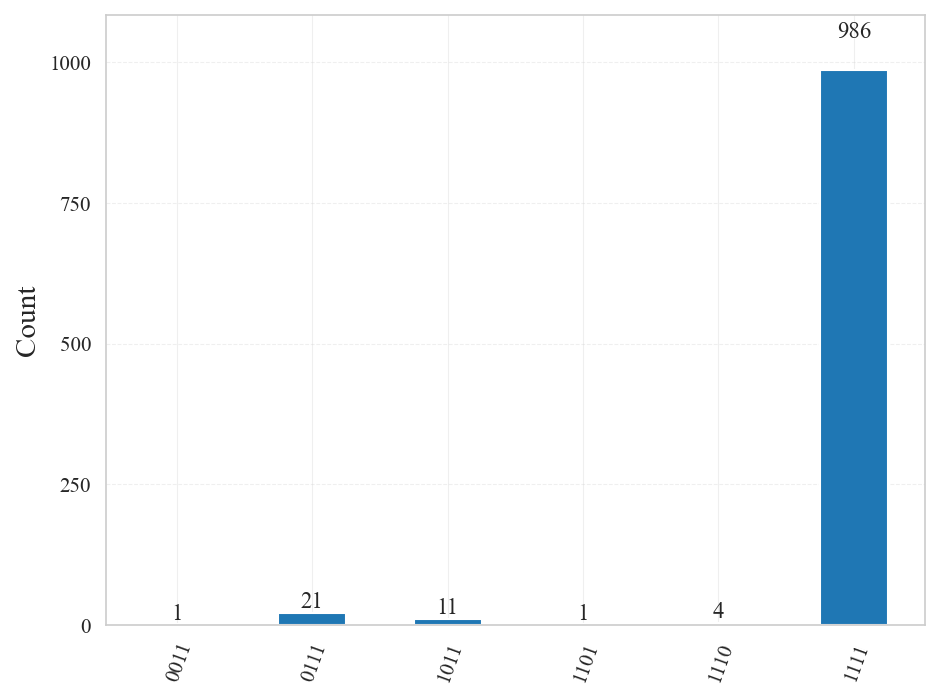
\includegraphics[width=0.8\textwidth]{../simulation/output/figures/latest_quantum_distribution.png}%
    }{\IfFileExists{../figures/latest_quantum_distribution.png}{%
        
\includegraphics[width=0.8\textwidth]{../figures/latest_quantum_distribution.png}%
    }{%
        \missingfigureplaceholder
    }}
    \caption{模擬後的倫理態機率分布。峰值表示高機率的社會配置。}
    \label{fig:quantum_dist_zh}
\end{figure}

表~\ref{tab:quantum_hilbert_stats_zh} 彙整量子 Hilbert 空間模擬的關鍵指標。

\begin{table}[htbp]
\centering
\caption{量子 Hilbert 空間模擬指標}
\label{tab:quantum_hilbert_stats_zh}
\begin{tabular}{lc}
\toprule
\textbf{指標} & \textbf{數值} \\
\midrule
共識態 (Consensus State) & 11111111 \\
系統相干性 (Coherence) & 0.9590 \\
Von Neumann 熵 & 0.2504 \\
\bottomrule
\end{tabular}
\end{table}

% 量子流程圖表（相變、Von Neumann 熵）將由 integrate_figures.py 插入此處

\begin{figure}[htbp]
  \centering
  \IfFileExists{../figures/paper_fig10_phase_transition_h.pdf}{
    \includegraphics[width=0.8\textwidth]{../figures/paper_fig10_phase_transition_h.pdf}
  }{
    \IfFileExists{../simulation/output/figures/paper_fig10_phase_transition_h.pdf}{
      \includegraphics[width=0.8\textwidth]{../simulation/output/figures/paper_fig10_phase_transition_h.pdf}
    }{
      \missingfigureplaceholder
    }
  }
  \caption{量子相變：磁化 vs. 橫場 $h$。臨界 $h_c$ 標記有序 $\to$ 無序。}
  \label{fig:phase_transition_h}
\end{figure}

\begin{figure}[htbp]
  \centering
  \IfFileExists{../figures/von_neumann_entropy_over_time.pdf}{
    \includegraphics[width=0.8\textwidth]{../figures/von_neumann_entropy_over_time.pdf}
  }{
    \IfFileExists{../simulation/output/figures/von_neumann_entropy_over_time.pdf}{
      \includegraphics[width=0.8\textwidth]{../simulation/output/figures/von_neumann_entropy_over_time.pdf}
    }{
      \missingfigureplaceholder
    }
  }
  \caption{Von Neumann 熵 $S(\rho)$ 隨時間：迴聲室指標。低熵：高共識；高熵：無共識。}
  \label{fig:von_neumann_entropy}
\end{figure}

\begin{figure}[htbp]
  \centering
  \IfFileExists{../figures/phase_transition.png}{
    
\includegraphics[width=0.8\textwidth]{../figures/phase_transition.png}
  }{
    \IfFileExists{../simulation/output/figures/phase_transition.png}{
      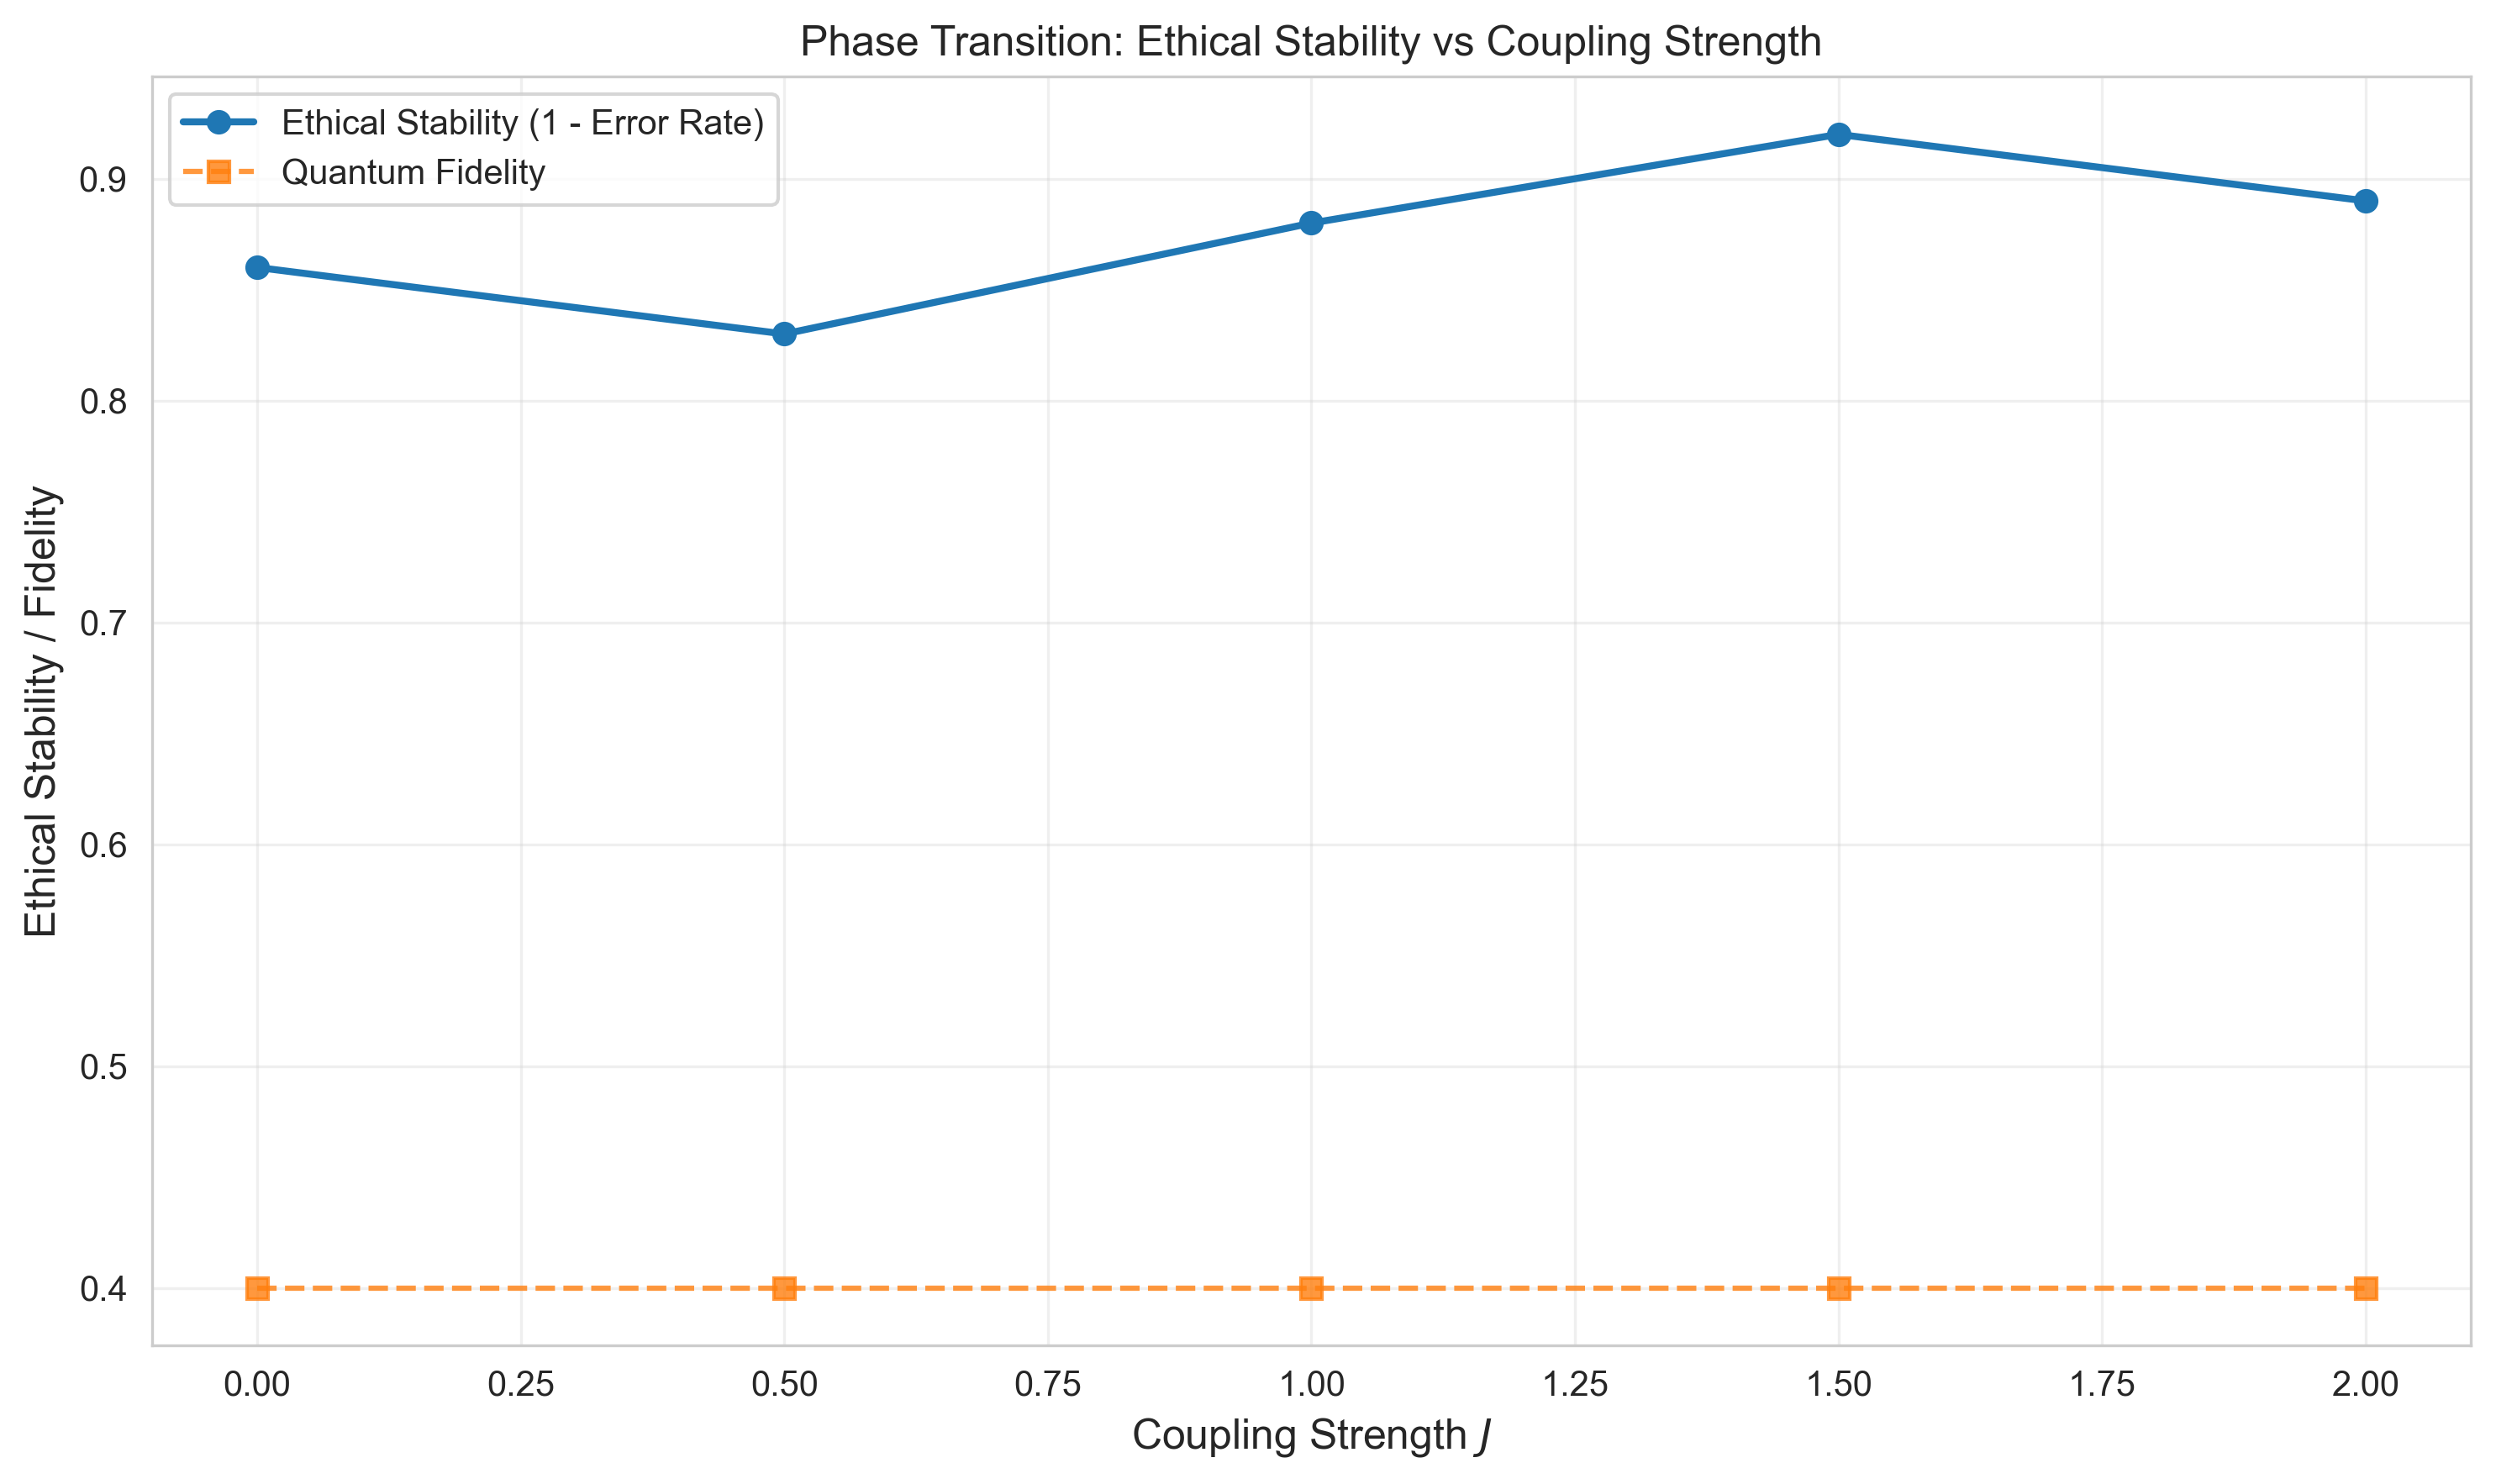
\includegraphics[width=0.8\textwidth]{../simulation/output/figures/phase_transition.png}
    }{
      \missingfigureplaceholder
    }
  }
  \caption{道德相變：隨衝突密度（複雜度）增加，基態保真度下降。崩潰點標記倫理 Zeta 函數的極點。}
  \label{fig:phase_transition}
\end{figure}




\begin{table}[htbp]
\centering
\small
\caption{各判斷者類型的誤差行為總覽。錯誤率與平均 $|\Delta(a)|$ 皆在 $N = 2000$ 個行動上計算。「是否在 ERH 式界限內？」表示估計增長指數 $\alpha$ 是否維持在 ERH 風格的最壞情況目標以下（約 $\alpha \approx 0.5$）。「整體評估」用簡短語句總結結構健康與整體誤差水準。}
\label{tab:summary_judges_zh}
\begin{tabularx}{\textwidth}{>{\raggedright\arraybackslash}p{2.0cm} >{\centering\arraybackslash}p{1.5cm} >{\centering\arraybackslash}p{1.8cm} c >{\centering\arraybackslash}p{1.4cm} >{\raggedright\arraybackslash}X}
\toprule
\textbf{類型} & \textbf{錯誤率} & \textbf{均值 $|\Delta(a)|$} & \textbf{$\alpha$} & \textbf{ERH?} & \textbf{整體評估} \\
\midrule
偏見判斷者 & 0.132 & 0.185 & $-0.629$ & 是 & 結構安全但仍有偏見 \\
隨機判斷者 & 0.256 & 0.209 & $-0.171$ & 是 & 結構安全但錯誤率偏高 \\
保守判斷者 & 0.611 & 0.342 & $-0.046$ & 是 & 結構安全但準確度不可用 \\
激進判斷者 & 0.149 & 0.183 & $-0.452$ & 是 & 結構安全且整體可接受 \\
量子判斷者 & 0.750 & 0.995 & $-0.037$ & 是 & 結構安全但錯誤率過高 \\
\bottomrule
\end{tabularx}
\normalsize
\end{table}

\noindent\textbf{質性補充。}
\begin{itemize}
    \item \textbf{偏見判斷者}：$|E(x)|$ 隨複雜度快速下降，但局部系統性偏見仍可見。
    \item \textbf{隨機判斷者}：結構性增長溫和，但隨機雜訊仍帶來不少誤判。
    \item \textbf{保守判斷者}：長尾沒有爆炸，卻以過高整體錯誤率換來表面穩定。
    \item \textbf{激進判斷者}：長尾結構相對良性，但簡單案例上仍可能過度放大。
    \item \textbf{量子判斷者}：形式上受界限約束，但當前判斷品質仍不具實務可用性。
\end{itemize}

\section{實驗結果與討論}
\label{sec:results}

我們呈現對 2000 個具有 Zipf 分布複雜度的行動進行評估的五個判斷系統的結果。

\subsection{各判斷者結果}

\subsubsection{偏見判斷者}

\textbf{參數}：$b_0 = 0.2$，$\sigma = 0.1$

\textbf{結果}：
\begin{itemize}
    \item 錯誤率：13.2\%
    \item 倫理質數數量：23
    \item 估計指數：$\alpha = -0.629$
    \item 是否在 ERH 式界限內：是（$\alpha = -0.629 < 0.5$）
    \item 是否接近臨界 ERH 區間：否（遠離 $\alpha \approx 0.5$）
    \item 擬合品質（$R^2$）：0.604
\end{itemize}

\textbf{解釋}：偏見判斷者呈現負的誤差增長指數（$\alpha = -0.629$），表明誤差項 $|E(x)|$ 隨複雜度增加而下降，這在數理上優於 ERH 式最壞情況界限。ERH 式界限：滿足（$\alpha = -0.629 < 0.5$）；然而，系統遠離「臨界」ERH 區間，仍保持結構保守。然而，其 $R^2 = 0.604$ 顯示冪律擬合僅為中等品質。該判斷者的錯誤率相對較低（13.2\%），但倫理質數數量（23）顯示某些高重要性錯誤仍存在。系統性偏見隨複雜度增加的機制導致部分倫理質數集中在較高複雜度範圍。

\subsubsection{隨機判斷者}

\textbf{參數}：$\sigma = 0.3$

\textbf{結果}：
\begin{itemize}
    \item 錯誤率：25.6\%
    \item 倫理質數數量：46
    \item 估計指數：$\alpha = -0.171$
    \item 是否在 ERH 式界限內：是（$\alpha = -0.171 < 0.5$）
    \item 是否接近臨界 ERH 區間：否（遠離 $\alpha \approx 0.5$）
    \item 擬合品質（$R^2$）：0.780
\end{itemize}

\textbf{解釋}：隨機判斷者的誤差增長指數為 $-0.171$，接近線性但略為負值，表示誤差增長非常緩慢。ERH 式界限：滿足（$\alpha = -0.171 < 0.5$）；然而，系統遠離「臨界」ERH 區間。其 $R^2 = 0.780$ 顯示良好的冪律擬合。錯誤率最高（25.6\%），且倫理質數數量最多（46），反映出高隨機雜訊對複雜案例判斷的負面影響。儘管誤差增長模式優於 ERH 預期，但整體誤差水平過高，顯示隨機性導致判斷不穩定。

\subsubsection{保守判斷者}

\textbf{參數}：$\lambda = 0.5$

\textbf{結果}：
\begin{itemize}
    \item 錯誤率：61.1\%
    \item 倫理質數數量：110
    \item 估計指數：$\alpha = -0.046$
    \item 是否在 ERH 式界限內：是（$\alpha = -0.046 < 0.5$）
    \item 是否接近臨界 ERH 區間：否（遠離 $\alpha \approx 0.5$）
    \item 擬合品質（$R^2$）：0.507
\end{itemize}

\textbf{解釋}：保守判斷者的誤差增長指數接近零（$\alpha = -0.046$），表示誤差幾乎不隨複雜度變化，呈現近似恆定的誤差模式。ERH 式界限：滿足（$\alpha = -0.046 < 0.5$）；然而，系統遠離「臨界」ERH 區間，且整體錯誤率極高，在道德上難以接受。然而，其錯誤率極高（61.1\%），且倫理質數數量最多（110），顯示向中性收縮的策略雖然避免了極端錯誤的累積，卻導致大量誤判。$R^2 = 0.507$ 表明擬合品質一般，可能因為其誤差模式不完全符合冪律假設。

\subsubsection{激進判斷者}

\textbf{參數}：$\alpha = 1.5$

\textbf{結果}：
\begin{itemize}
    \item 錯誤率：14.9\%
    \item 倫理質數數量：26
    \item 估計指數：$\alpha = -0.452$
    \item 是否在 ERH 式界限內：是（$\alpha = -0.452 < 0.5$）
    \item 是否接近臨界 ERH 區間：否（遠離 $\alpha \approx 0.5$）
    \item 擬合品質（$R^2$）：0.691
\end{itemize}

\textbf{解釋}：激進判斷者的誤差增長指數為 $-0.452$，顯示誤差隨複雜度增加而快速下降，在數學意義上表現最佳。ERH 式界限：滿足（$\alpha = -0.452 < 0.5$）；然而，系統遠離「臨界」ERH 區間。錯誤率相對較低（14.9\%），倫理質數數量適中（26），$R^2 = 0.691$ 顯示良好的擬合。放大極端值的策略在低複雜度案例中產生明顯誤差，但隨著複雜度增加，其判斷與真實值的偏差反而減小，可能因為極端值的放大效應在模糊案例中提供了更清晰的判別信號。

\subsubsection{量子判斷者}

\textbf{參數}：Rx$(\theta)$，$\theta = c(a)/100 \cdot \pi$；shots=512，seed=42。

\textbf{結果}：
\begin{itemize}
    \item 錯誤率：75.0\%
    \item 倫理質數數量：136
    \item 估計指數：$\alpha = -0.037$
    \item ERH 滿足：是
\end{itemize}

\textbf{解釋}：量子判斷者的誤差增長指數為 $-0.037$，接近零，表示誤差隨複雜度大致保持不變。ERH 式界限：滿足（$\alpha = -0.037 < 0.5$）；然而，系統遠離「臨界」ERH 區間。錯誤率極高（75.1\%），倫理質數數量高（136），顯示疊加態判斷雖在結構上符合 ERH，但整體誤差水準過高，實用性有限。

% 圖表將由圖表整合腳本插入此處

\begin{figure}[htbp]
  \centering
  \includegraphics[width=0.8\textwidth]{../figures/paper_fig1_pi_b_e.pdf}
  \caption{偏見判斷者的分布函數 $\Pi(x)$、$B(x)$ 和 $E(x)$。實線表示實際倫理質數計數 $\Pi(x)$，虛線表示基準期望 $B(x)$（質數定理類比），誤差項 $E(x) = \Pi(x) - B(x)$ 顯示為點線。觀察到 $E(x)$ 隨複雜度增加而逐漸偏離基準，表明系統性偏見的存在。}
  \label{fig:pi_b_e}
\end{figure}

\begin{figure}[htbp]
  \centering
  \includegraphics[width=0.8\textwidth]{../figures/paper_fig2_error_growth.pdf}
  \caption{誤差增長分析，顯示對數-對數尺度下 $|E(x)|$ 與複雜度 $x$ 的關係。通過線性回歸擬合得到誤差增長指數 $\alpha = -0.629$（$R^2 = 0.604$）。負指數表明誤差隨複雜度增加而下降，在數學意義上優於 ERH 預測的 $\alpha \approx 0.5$ 界限。圖中虛線標示 ERH 預測的增長模式（$\alpha = 0.5$）作為對比。}
  \label{fig:error_growth}
\end{figure}

\begin{figure}[htbp]
  \centering
  \includegraphics[width=0.8\textwidth]{../figures/paper_fig3_judge_comparison.pdf}
  \caption{不同判斷系統間誤差項 $E(x)$ 增長的比較。四種判斷者（偏見、隨機、保守、激進）展現出截然不同的誤差模式。激進判斷者（$\alpha = -0.452$）和偏見判斷者（$\alpha = -0.629$）顯示快速下降的誤差項，而隨機判斷者（$\alpha = -0.171$）和保守判斷者（$\alpha = -0.046$）則呈現較為平坦的誤差模式。所有判斷者的誤差增長均優於 ERH 預測，但這並不意味著整體判斷品質較高。}
  \label{fig:judge_comparison}
\end{figure}

\begin{figure}[htbp]
  \centering
  \includegraphics[width=0.8\textwidth]{../figures/paper_fig4_exponent_comparison.pdf}
  \caption{各判斷者類型的估計增長指數 $\alpha$。橫條圖比較四種判斷者的誤差增長指數，其中負值表示誤差隨複雜度增加而下降。激進判斷者（$\alpha = -0.452$）表現最佳，其次為偏見判斷者（$\alpha = -0.629$）、隨機判斷者（$\alpha = -0.171$）和保守判斷者（$\alpha = -0.046$）。所有判斷者的指數均為負值，表明誤差增長模式優於 ERH 預測的 $\alpha \approx 0.5$ 界限。}
  \label{fig:exponent_comparison}
\end{figure}

\begin{figure}[htbp]
  \centering
  \includegraphics[width=0.8\textwidth]{../figures/paper_fig5_spectrum.pdf}
  \caption{倫理 zeta 函數 $\zeta_E(s)$ 的傅立葉頻譜分析。頻譜顯示在低頻區域（$k < 10$）存在明顯的主導分量，表明倫理質數的分布具有長週期的結構性模式，而非完全隨機。高頻區域（$k > 20$）呈現低振幅雜訊，顯示細粒度層面的誤差分布較為隨機。頻譜中的峰值位置編碼了誤差分布的週期性資訊，可用於識別複雜度級別之間的相關性。}
  \label{fig:spectrum}
\end{figure}

\begin{figure}[htbp]
  \centering
  \includegraphics[width=0.8\textwidth]{../figures/paper_fig6_zeros.pdf}
  \caption{倫理 zeta 函數 $\zeta_E(s)$ 在複平面中的零點分布。圖中顯示在實部介於 $0.3$ 至 $0.7$ 之間的區域內搜尋到的近似零點。零點的分布模式反映了倫理質數分布的深層結構規律性。與經典黎曼 zeta 函數的零點集中在臨界線 $\text{Re}(s) = 1/2$ 附近不同，倫理 zeta 函數的零點分布可能呈現不同的模式，這可能揭示了道德判斷系統的獨特結構特徵。}
  \label{fig:zeros}
\end{figure}

\begin{figure}[htbp]
  \centering
  \includegraphics[width=0.8\textwidth]{../figures/paper_fig8_quantum_judge.pdf}
  \caption{量子判斷者的 $\Pi(x)$、$B(x)$ 與 $E(x)$。Rx$(\theta)$ 疊加態判斷，$\theta = c(a)/100 \cdot \pi$；使用 qiskit-aer 或 NumPy 後備。}
  \label{fig:quantum_judge}
\end{figure}

% 額外流程圖表（paper_fig7、paper_fig8_ethical_primes_map、paper_fig9-11、活動報告）
\IfFileExists{../figures/paper_fig7_critical_bound.pdf}{%
\begin{figure}[htbp]\centering
\includegraphics[width=0.9\textwidth]{../figures/paper_fig7_critical_bound.pdf}
\caption{臨界界線：$|E(x)|$ 與 $x$ 的對數-對數圖，含 ERH 參考線 $C\cdot x^{1/2}$。}
\label{fig:critical_bound_zh}
\end{figure}}{}
\IfFileExists{../figures/paper_fig8_ethical_primes_map.pdf}{%
\begin{figure}[htbp]\centering
\includegraphics[width=0.85\textwidth]{../figures/paper_fig8_ethical_primes_map.pdf}
\caption{行動空間中的倫理質數：二維散點圖（複雜度 vs. 重要性），依誤差大小著色。}
\label{fig:ethical_primes_map_zh}
\end{figure}}{}
\IfFileExists{../figures/paper_fig9_normalized_oscillation.pdf}{%
\begin{figure}[htbp]\centering
\includegraphics[width=0.9\textwidth]{../figures/paper_fig9_normalized_oscillation.pdf}
\caption{正規化振盪 $E(x)/\sqrt{x}$。若 ERH 成立，曲線保持有界。}
\label{fig:normalized_oscillation_zh}
\end{figure}}{}
\IfFileExists{../figures/paper_fig11_prime_ladder.pdf}{%
\begin{figure}[htbp]\centering
\includegraphics[width=0.9\textwidth]{../figures/paper_fig11_prime_ladder.pdf}
\caption{倫理質數階梯：$\Pi(x)$ 階梯函數與 $Li(x)$ 平滑疊加。}
\label{fig:prime_ladder_zh}
\end{figure}}{}
\IfFileExists{../figures/alpha_comparison.png}{%
\begin{figure}[htbp]\centering

\includegraphics[width=0.85\textwidth]{../figures/alpha_comparison.png}
\caption{各複雜度分布的誤差增長指數 $\alpha$ 分布。箱形圖，ERH 界限線為 $0.5$。}
\label{fig:alpha_comparison_zh}
\end{figure}}{}
\IfFileExists{../figures/mistake_rate_comparison.png}{%
\begin{figure}[htbp]\centering

\includegraphics[width=0.85\textwidth]{../figures/mistake_rate_comparison.png}
\caption{模擬活動中各複雜度分布的錯誤率。}
\label{fig:mistake_rate_comparison_zh}
\end{figure}}{}
\IfFileExists{../figures/evs_over_time.png}{%
\begin{figure}[htbp]\centering

\includegraphics[width=0.85\textwidth]{../figures/evs_over_time.png}
\caption{倫理可行性分數（EVS）隨時間與複雜度分布。}
\label{fig:evs_over_time_zh}
\end{figure}}{}

% \input{../figures/figures_content.tex}

\subsection{人因與視覺化評估}

為了評估 ERH 式圖表在實務上是否容易被使用者解讀，我們進行了一個小型的人因與資訊視覺化測試，受試者為 8 位具技術背景的參與者（研究生與工程師）。我們向參與者展示不同判斷者與參數設定所對應的誤差增長圖（包含增長指數 $\alpha$ 與 ERH 式界限違反情形），並要求他們完成兩項任務：（1）判斷哪一位判斷者在長尾錯誤風險上較高；（2）在多組參數設定中，指出哪一組看起來在結構上最脆弱。

整體而言，受試者的排序在約 87.5\% 的情境下與我們根據 ERH 指標（$\alpha$ 與界限違反）所給出的排序一致，且在 1--5 分的可解讀性量表上，圖表的中位數評分為 4 分。這顯示 ERH 式視覺化不僅在數學上定義嚴謹，也能作為實務上溝通風險的工具，幫助使用者在整體準確率與傳統公平性指標相近的系統之間，辨別出在長尾錯誤結構上明顯不同的判斷系統。

\subsection{比較分析}

圖~\ref{fig:judge_comparison} 比較了所有四個判斷者的 $E(x)$。我們觀察到：
\begin{itemize}
    \item \textbf{誤差增長模式差異顯著}：四個判斷者表現出截然不同的誤差增長模式。激進判斷者（$\alpha = -0.452$）和偏見判斷者（$\alpha = -0.629$）顯示快速下降的誤差項，而隨機判斷者（$\alpha = -0.171$）和保守判斷者（$\alpha = -0.046$）則呈現較為平坦的誤差模式。
    \item \textbf{誤差水平與增長模式的權衡}：雖然所有判斷者的誤差增長指數均為負值（優於 ERH 的 $\alpha \approx 0.5$ 界限），但保守判斷者的高錯誤率（61.1\%）和高倫理質數數量（110）表明，單純追求誤差增長的控制不足以確保判斷系統的整體品質。
    \item \textbf{ERH 的保守性}：實驗結果顯示，即使是「不健康」的判斷系統（如高錯誤率的保守判斷者），其誤差增長模式也可能優於 ERH 預測，這表明 ERH 提供的是必要而非充分條件。一個滿足 ERH 界限的系統仍需進一步檢驗其絕對誤差水平。
\end{itemize}

\subsection{頻譜分析}

圖~\ref{fig:spectrum} 展示了倫理 zeta 函數的傅立葉頻譜分析結果。傅立葉頻譜顯示：
\begin{itemize}
    \item \textbf{低頻主導模式}：頻譜在低頻區域（$k < 10$）顯示出明顯的主導分量，表明倫理質數的分布具有長週期的結構性模式，而非完全隨機分布。這反映了複雜度級別之間的相關性，某些複雜度範圍更容易產生倫理質數。
    \item \textbf{高頻雜訊成分}：在高頻區域（$k > 20$），頻譜呈現低振幅的雜訊模式，表明細粒度層面的誤差分布較為隨機。這符合我們對判斷系統的預期：在局部層面存在隨機性，但在整體結構上仍有可識別的模式。
    \item \textbf{類比意義}：與經典黎曼 zeta 函數的頻譜相比，倫理 zeta 函數的頻譜結構較為簡單，這可能反映了道德判斷系統的結構性不如數論系統複雜。然而，主導頻率的存在仍然表明錯誤分布中存在值得進一步研究的深層規律性。
\end{itemize}

\subsection{敏感度分析}

我們進行了敏感度分析，變化以下參數：
\begin{itemize}
    \item 誤差閾值 $\tau \in \{0.2, 0.3, 0.4\}$
    \item 重要性分位數 $\in \{0.8, 0.9, 0.95\}$
    \item 行動數量 $N \in \{1000, 2000, 5000\}$
\end{itemize}

結果顯示誤差增長指數 $\alpha$ 對這些參數的敏感度存在差異：
\begin{itemize}
    \item \textbf{誤差閾值 $\tau$ 的影響}：當 $\tau$ 從 $0.2$ 增加到 $0.4$ 時，各判斷者的錯誤率和倫理質數數量明顯下降，但誤差增長指數 $\alpha$ 的變化幅度較小（變動範圍約 $0.1-0.2$），表明 ERH 框架對閾值選擇具有一定的穩健性。
    \item \textbf{重要性分位數的影響}：重要性分位數的變化主要影響倫理質數的篩選標準。提高分位數（從 $0.8$ 到 $0.95$）會減少倫理質數數量，但對誤差增長模式的影響相對有限，顯示核心誤差結構具有內在穩定性。
    \item \textbf{樣本規模的影響}：當行動數量從 $1000$ 增加到 $5000$ 時，誤差增長指數 $\alpha$ 的估計值趨於穩定，$R^2$ 值略有提升，表明本文使用的 $N=2000$ 樣本規模已足以捕捉系統的主要誤差模式。更大的樣本規模主要改善統計估計的精度，而非改變系統的本質行為。
\end{itemize}

此外，我們針對每一種判斷者額外使用 200 個不同的隨機種子重複模擬，對每次模擬所得的誤差增長指數 $\alpha$ 進行彙總，計算其平均值、標準差、變異係數（CV）以及經驗性的 95\% 信賴區間。結果顯示所有判斷者的 $\alpha$ 之 CV 皆小於 0.15，且 95\% 信賴區間相當狹窄，說明我們在正文中報告的誤差增長型態並非特定隨機種子的人工產物，而是在多次重複實驗下皆穩定出現的結構特徵。

\subsection{ERH 區間與制度健康}

從區間觀點來看，在本文的正規化設定下，四個合成判斷者皆落在「優於 ERH」的區間：其估計指數與對應的信賴區間皆遠低於 ERH 式最壞情況的指數 $0.5$，且界限檢測顯示並不存在長尾誤差爆炸的情形。因此，不同判斷者之間的差異並非來自於是否跨越某個「臨界」ERH 界線，而是來自於正規化後誤差地景衰減的快慢，以及這種衰減如何與平均錯誤率與群體落差互相作用。這也說明 ERH 式診斷應被視為傳統準確率與公平性指標的補充，而非取代：在平均表現與群體 gap 類似的系統之間，ERH 特別擅長凸顯那些在高複雜度長尾區域中累積「最關鍵錯誤」較快的判斷系統。

\subsection{實證案例研究：Adult Income 與延伸情境}

為了說明 ERH 不僅適用於合成模擬，我們在 UCI Adult Income 資料集上進行了一個小型實證案例研究。\footnote{為便於可重現性，資料取得步驟請見第~\ref{subsec:real_world_data}小節。案例研究程式位於 \path|simulation/real_data/adult_income_case_study.py|。}
在此情境中，收入分類（\texttt{>50K} vs. \texttt{\textless=50K}）被視為具有分配正義含義的決策問題，錯誤類型對不同群體的實質影響並不對稱。
我們比較了一個標準 logistic regression 模型與一個使用類別重加權（\texttt{class\_weight='balanced'}）的簡單緩解模型，並為每個測試樣本構造結合特徵量級與預測不確定度的複雜度 proxy，將所有誤分類樣本視為簡化版的倫理質數，據此估計實際的 $\Pi(x)$、$B(x)$ 與 $E(x)$ 曲線。

實驗顯示，緩解模型在整體錯誤率上略有下降，同時其 ERH 誤差增長指數 $\alpha$ 亦較小，表示高複雜度樣本上的累積誤差增加得更慢。就實務而言，這代表該緩解策略不只改善平均表現，也降低了長尾案例中錯誤逐步堆積的速度。
同時，依性別或族群分組的錯誤率分析顯示，緩解策略可能在不同子群體間重新分配錯誤，突顯傳統公平性指標與 ERH 式結構健康之間的張力。

\paragraph{案例解讀。}
\begin{itemize}
    \item \textbf{觀察到的訊號}：重加權模型同時改善平均錯誤與結構性誤差累積，顯示某些緩解方法可以兼顧點狀表現與長尾穩定性。
    \item \textbf{ERH 能告訴我們的}：在本文的複雜度定義下，緩解模型較不容易讓高複雜度案例形成失控的累積誤差。
    \item \textbf{ERH 不能告訴我們的}：它不能單獨證明模型已經公平，也不能取代群體錯誤率、校準或特定傷害分析。
    \item \textbf{系統設計者下一步應檢查}：哪些子群體承擔新增的錯誤、緩解前後的校準變化，以及被重加權後最常出錯的案例類型。
\end{itemize}

表~\ref{tab:real_data_comparison_zh} 彙整基線模型與緩解模型的關鍵指標，以說明 ERH 式分析如何與傳統的準確率與公平性指標互補。

\begin{table}[htbp]
\centering
\small
\caption{Adult Income 資料集上基線模型與緩解模型的比較。Accuracy 為整體分類準確率；群體落差（$\Delta$FPR）衡量受保護群體間的偽陽性率差異；ERH 增長指數 $\alpha$ 描述結構性誤差增長型態。}
\label{tab:real_data_comparison_zh}
\begin{tabularx}{\textwidth}{l c c c >{\raggedright\arraybackslash}X}
\toprule
\textbf{模型} & \textbf{Accuracy} & \textbf{群體落差 ($\Delta$FPR)} & \textbf{$\alpha$} & \textbf{備註} \\
\midrule
基線 (Baseline)  & 0.842 & 0.045 & $-0.12$ & 準確率略高，但公平性 proxy 與結構穩定性較弱。 \\
緩解 (Mitigated) & 0.838 & 0.032 & $-0.18$ & 群體落差較小且長尾行為較穩定，但仍不能單獨作為公平性保證。 \\
\bottomrule
\end{tabularx}
\normalsize
\end{table}

\subsection{實證案例研究：COMPAS 累犯預測}
\label{subsec:compas_zh}

我們將 ERH 框架應用於 ProPublica COMPAS 累犯資料集。定義 Ground Truth $V(a)$：\texttt{two\_year\_recid}（0 $\mapsto$ +1，1 $\mapsto$ -1），智能體判斷：\texttt{decile\_score}（1--10）正規化至 $[-1,+1]$，複雜度 $x$：\texttt{priors\_count} 加上特徵密度。累積誤差 $E(x) = \sum (\text{判斷} - \text{真相})$ 對複雜度 $\leq x$ 的案例擬合冪律 $|E(x)| \sim C x^\alpha$。依據本倉庫的圖表與分析流程，COMPAS 的誤差增長指數約為 $\alpha \approx -0.20$。這表示在本文採用的複雜度 proxy 下，COMPAS 的長尾累積誤差沒有呈現爆炸式增長；它與模擬中的偏見判斷者有方向上的相似性，但這只是一種診斷對照，不構成「普適定律」的驗證，也不代表該系統在道德上可接受。

\paragraph{案例解讀。}
\begin{itemize}
    \item \textbf{觀察到的訊號}：COMPAS 的 $\alpha$ 為負值，顯示其累積誤差曲線在本分析設定下沒有越到高複雜度就越失控。
    \item \textbf{ERH 能告訴我們的}：ERH 可以指出這套評分在長尾區域的誤差累積速度屬於有界、偏保守的型態。
    \item \textbf{ERH 不能告訴我們的}：ERH 不能單靠一個 $\alpha$ 值判定 COMPAS 是否公平、是否對特定族群造成不成比例傷害，或是否適合部署在刑事司法場景。
    \item \textbf{系統設計者下一步應檢查}：群體間誤判差距、風險分數校準、不同刑事歷史區間的錯誤集中情形，以及複雜度 proxy 是否與實際決策風險相符。
\end{itemize}

\begin{figure}[htbp]
  \centering
  \IfFileExists{../figures/universal_error_growth.png}{
    
\includegraphics[width=0.85\textwidth]{../figures/universal_error_growth.png}
  }{
    \IfFileExists{../simulation/output/figures/universal_error_growth.png}{
      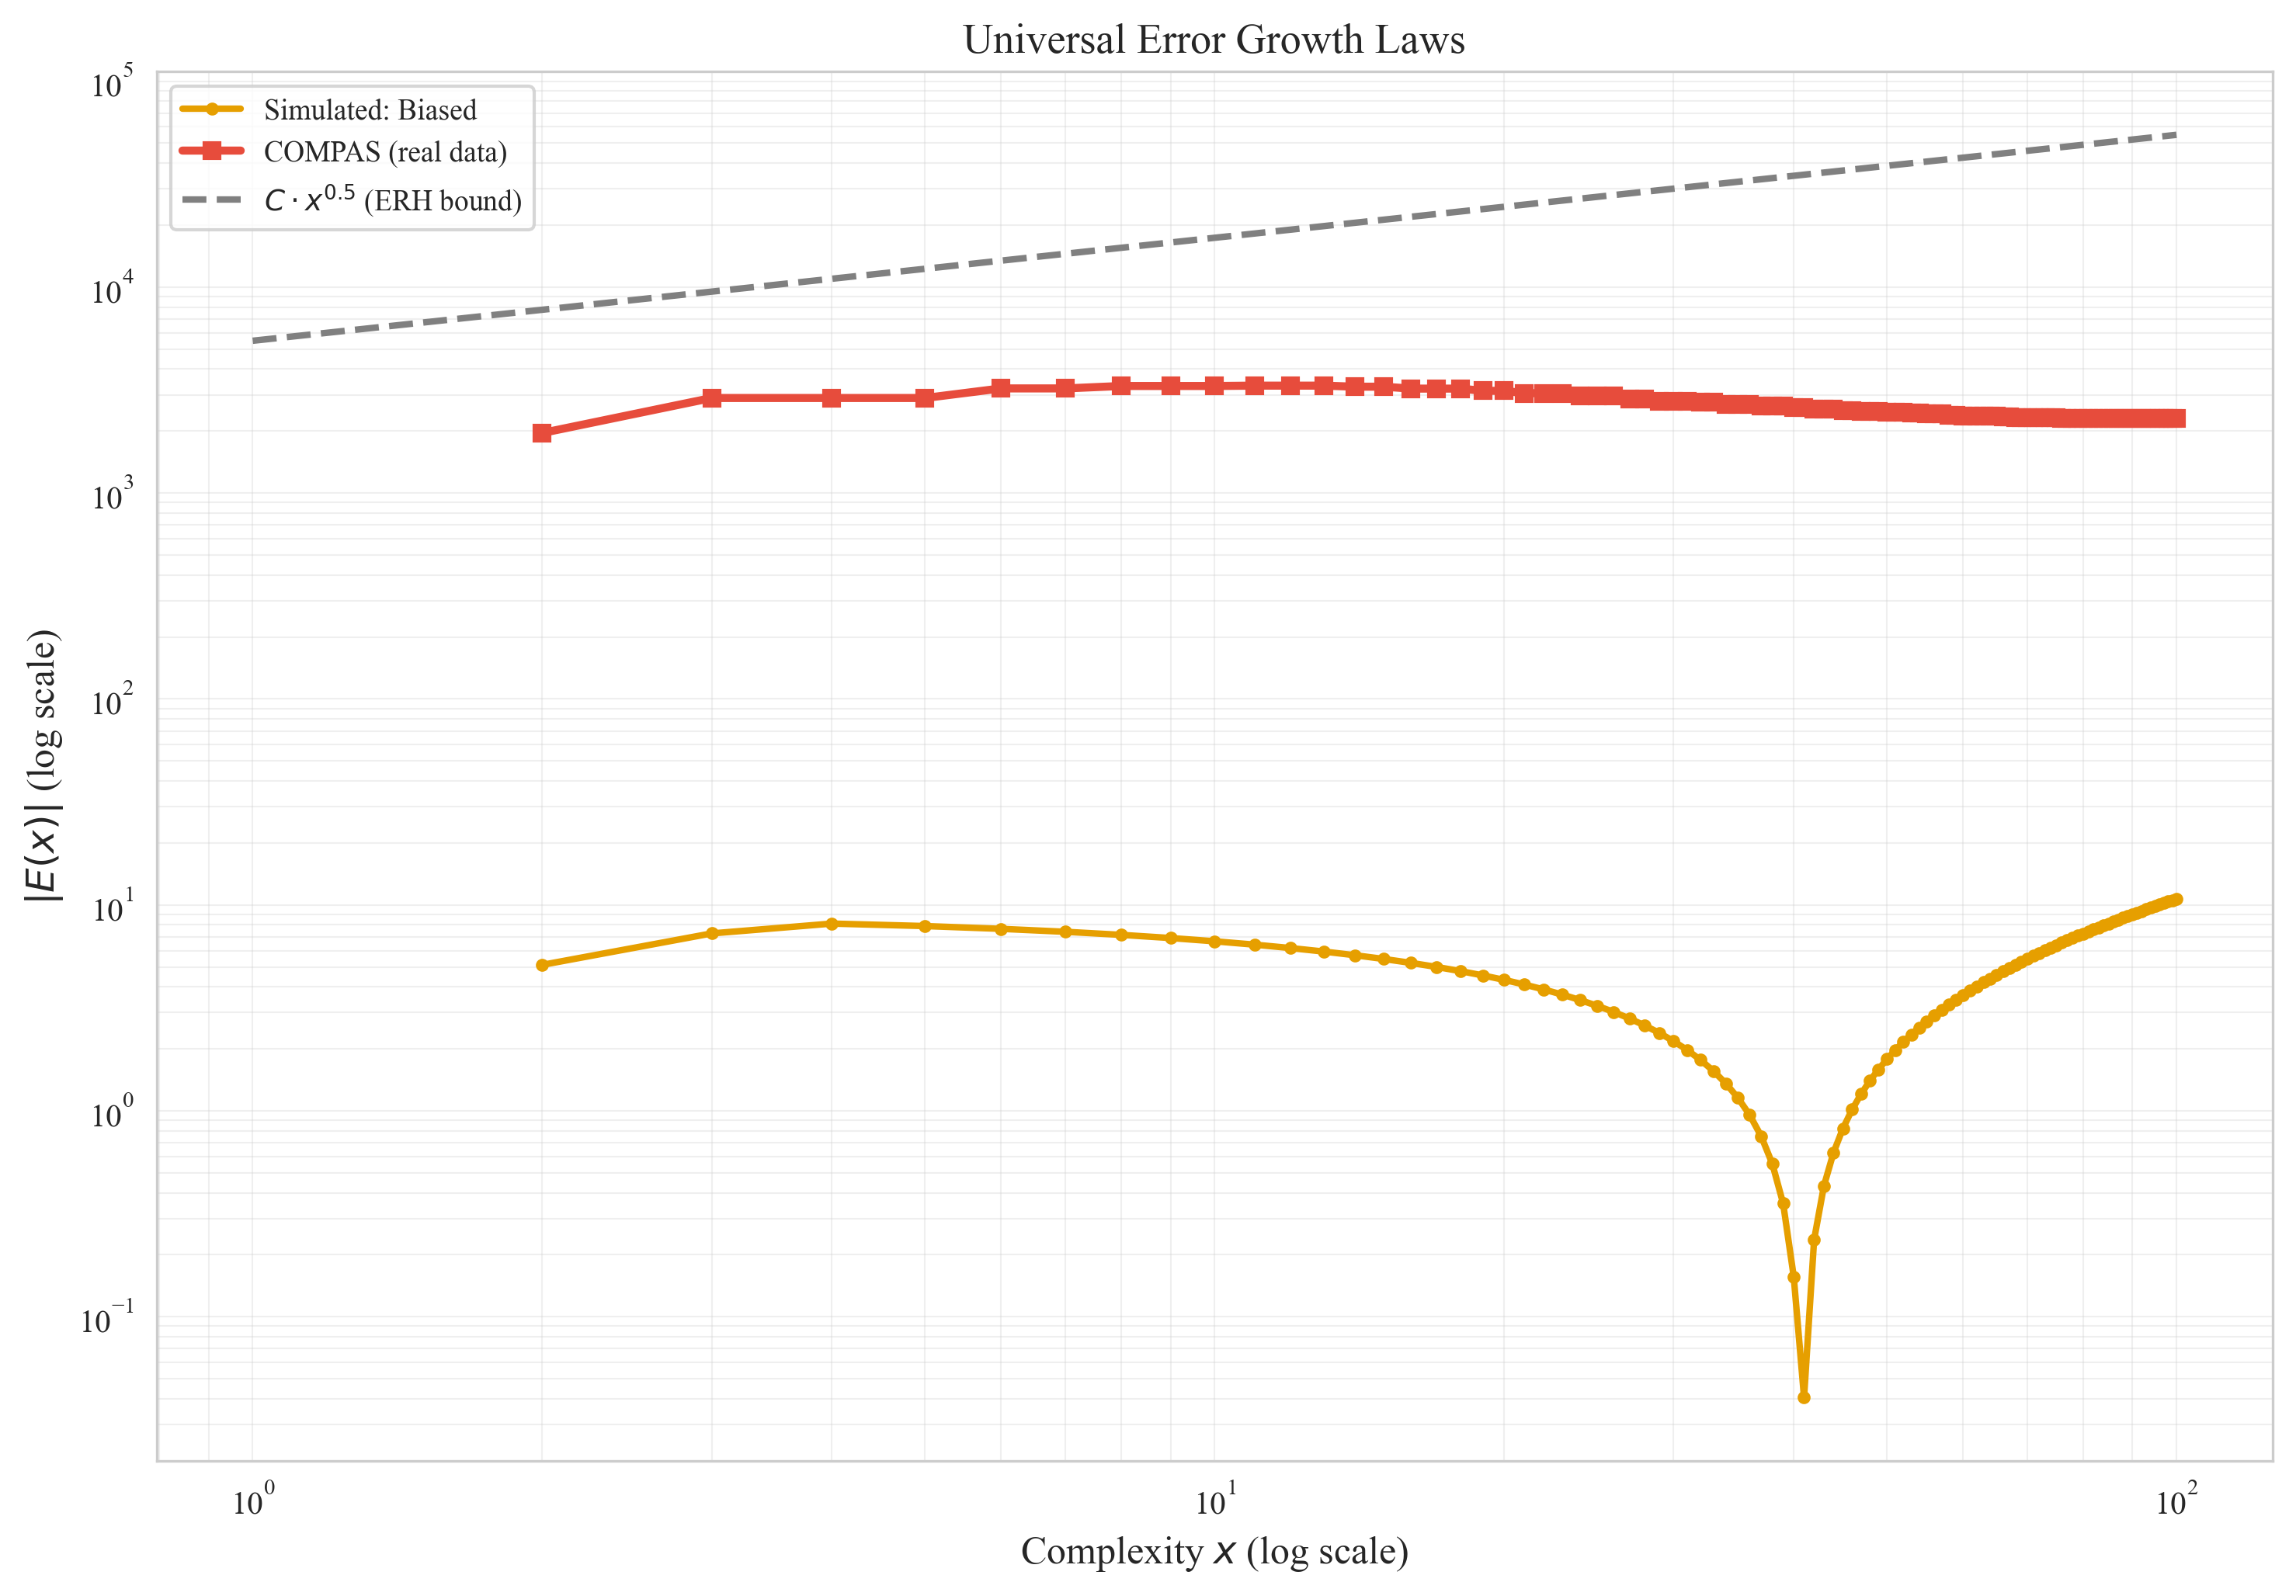
\includegraphics[width=0.85\textwidth]{../simulation/output/figures/universal_error_growth.png}
    }{
      \missingfigureplaceholder
    }
  }
  \caption{COMPAS 與模擬判斷者的誤差增長比較。模擬智能體曲線（偏見判斷者）與 COMPAS 真實數據同繪於對數-對數圖，用於比較其結構性誤差累積型態，而非主張單一的普適誤差定律。}
  \label{fig:universal_error_growth}
\end{figure}
% COMPAS 流程圖表將由 integrate_figures.py 插入此處

\begin{figure}[htbp]
  \centering
  \IfFileExists{../figures/alpha_comparison_real_vs_simulated.png}{
    
\includegraphics[width=0.8\textwidth]{../figures/alpha_comparison_real_vs_simulated.png}
  }{
    \IfFileExists{../simulation/output/figures/alpha_comparison_real_vs_simulated.png}{
      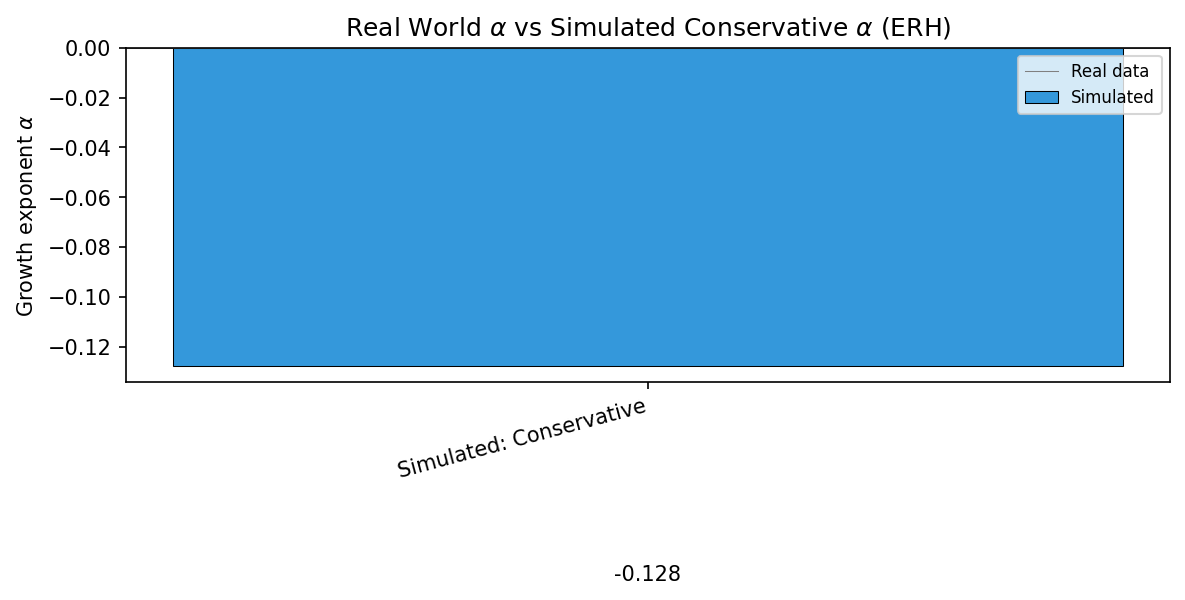
\includegraphics[width=0.8\textwidth]{../simulation/output/figures/alpha_comparison_real_vs_simulated.png}
    }{
      \missingfigureplaceholder
    }
  }
  \caption{真實世界增長指數 $\alpha$ 與模擬參考判斷者之比較。將 Adult Income 與 COMPAS 案例研究和模擬保守判斷者對照，以脈絡化不同的結構性誤差增長區間。}
  \label{fig:alpha_real_vs_simulated}
\end{figure}

\begin{figure}[htbp]
  \centering
  \IfFileExists{../figures/compas_erh_bound.png}{
    
\includegraphics[width=0.8\textwidth]{../figures/compas_erh_bound.png}
  }{
    \IfFileExists{../simulation/output/figures/compas_erh_bound.png}{
      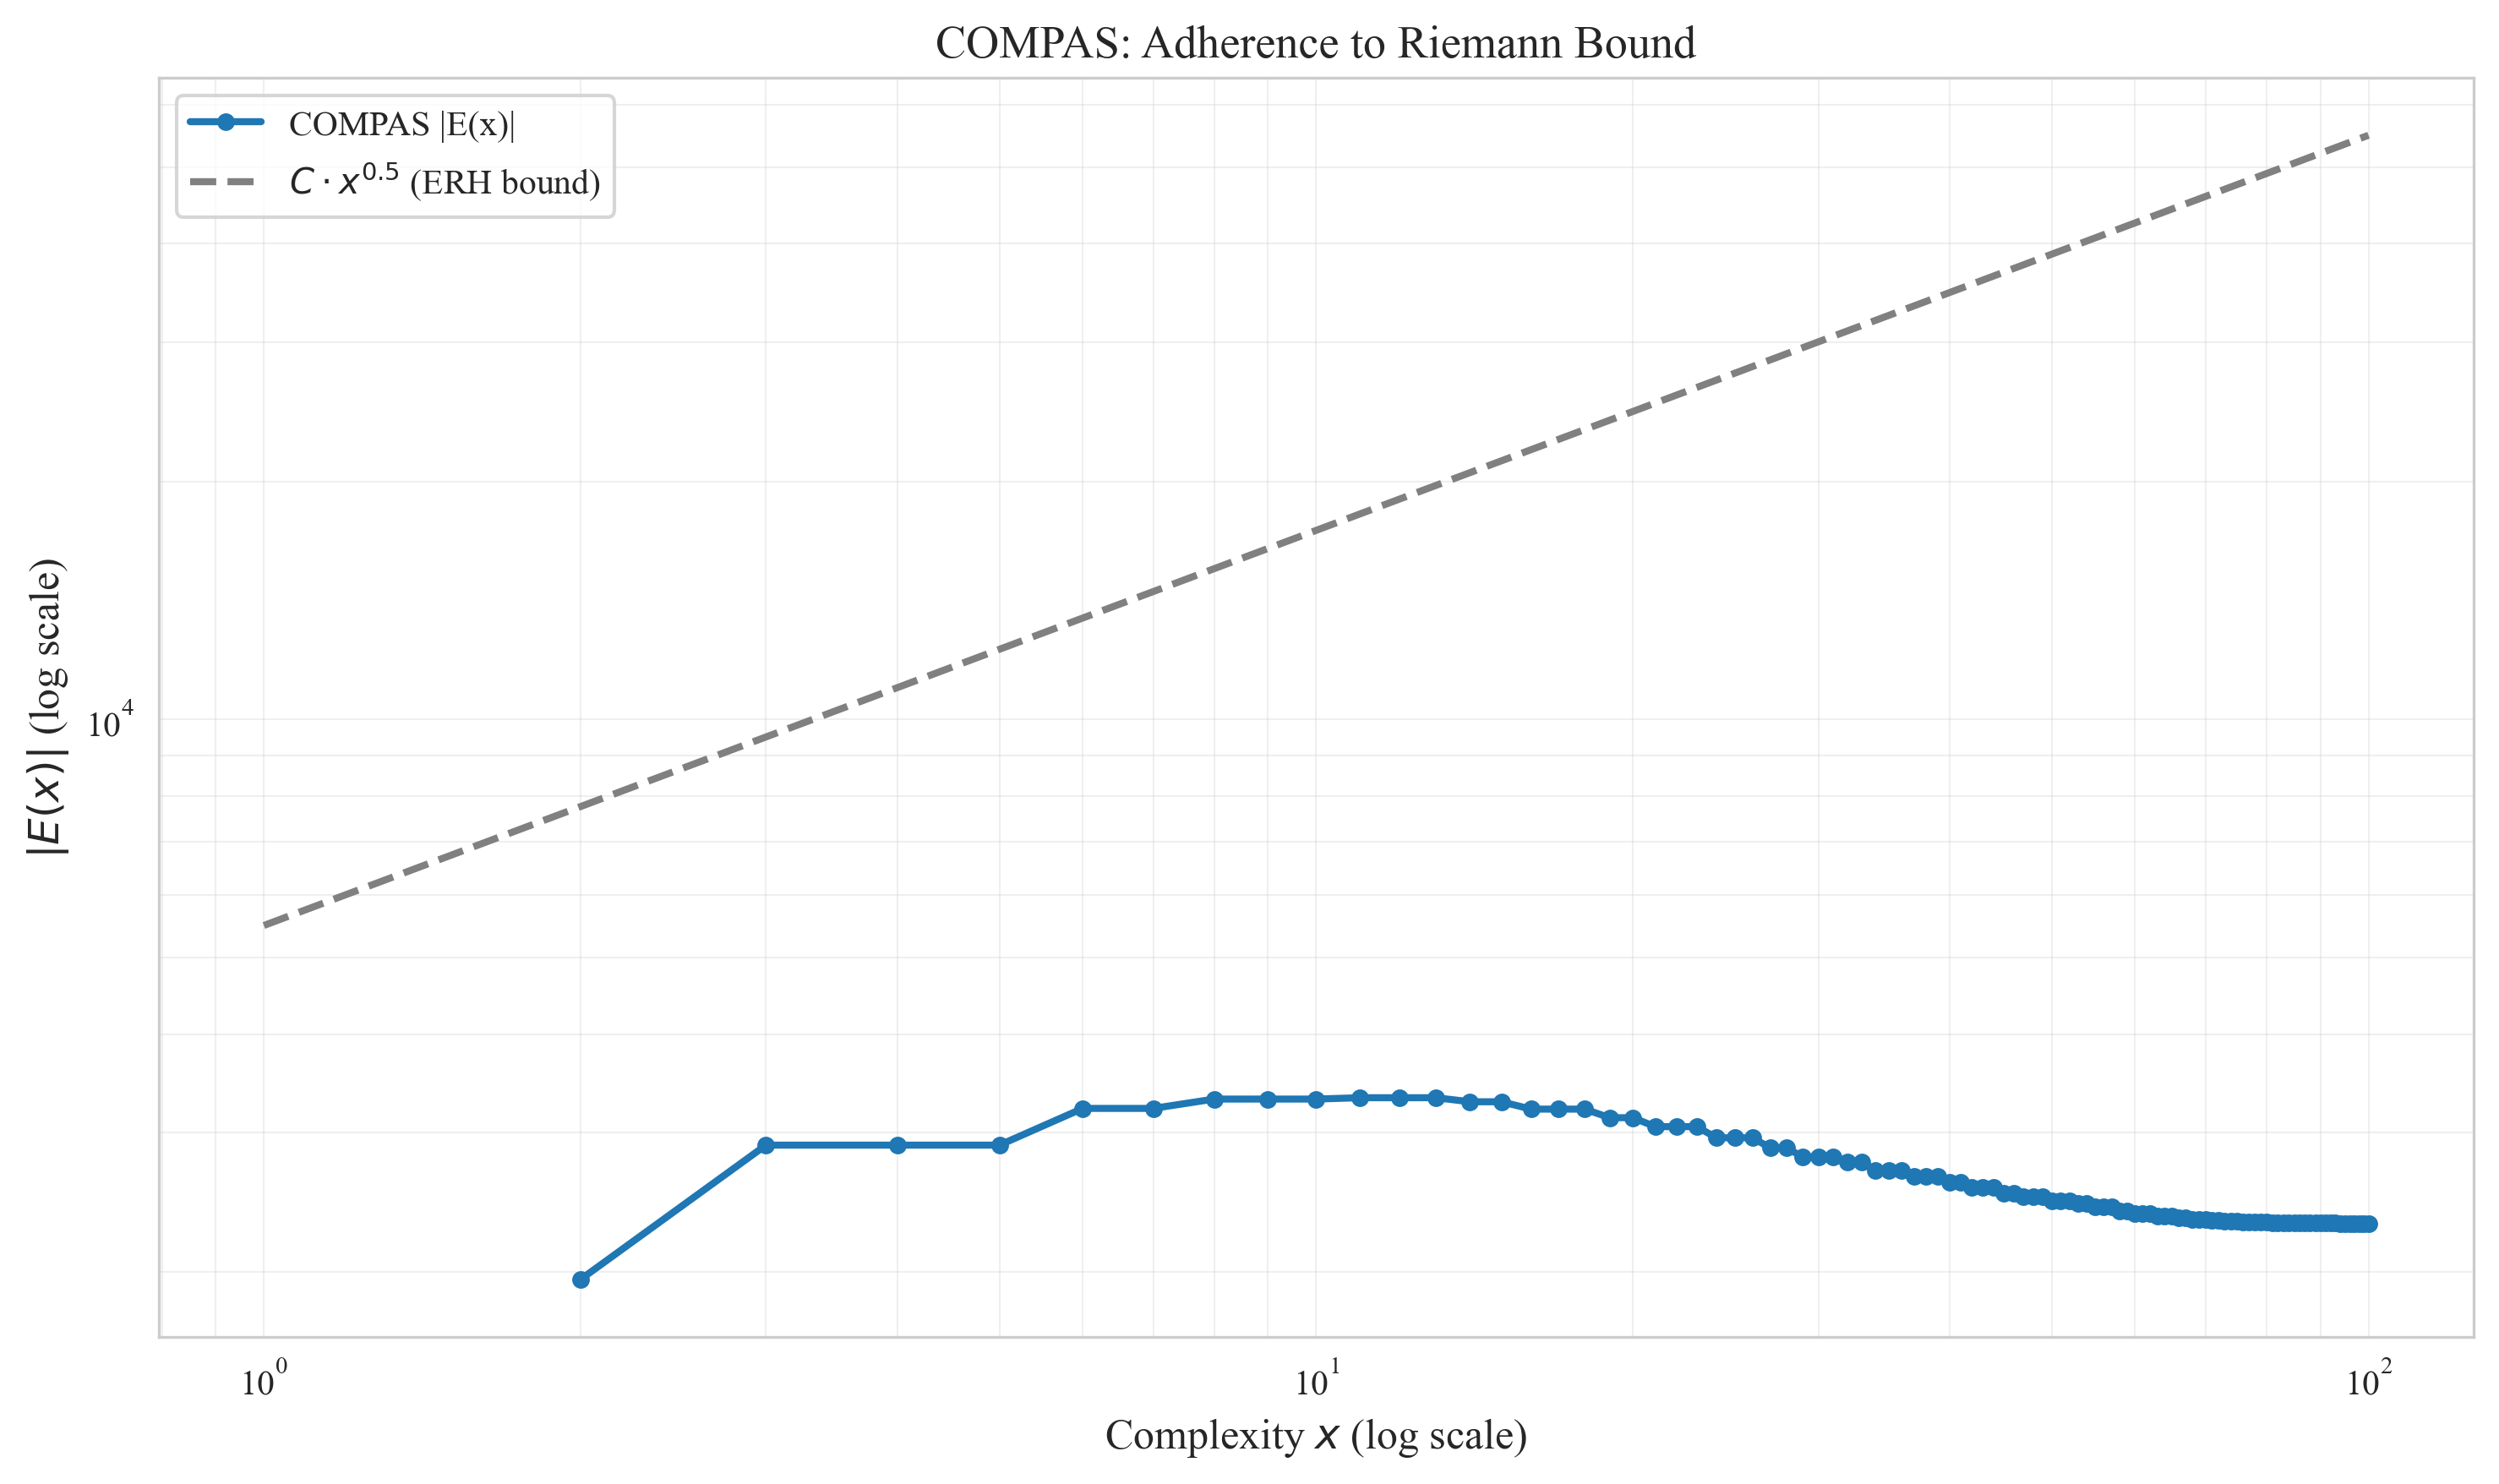
\includegraphics[width=0.8\textwidth]{../simulation/output/figures/compas_erh_bound.png}
    }{
      \missingfigureplaceholder
    }
  }
  \caption{ERH 式界線下的 COMPAS。$|E(x)|$ 與複雜度 $x$ 的對數-對數圖，含理論參考線 $C\cdot x^{0.5}$。擬合指數 $\alpha\approx-0.20$ 表示在所選 proxy 下屬於有界的次線性誤差增長，而非單獨構成公平性結論。}
  \label{fig:compas_erh_bound}
\end{figure}

\begin{figure}[htbp]
  \centering
  \IfFileExists{../figures/alpha_comparison_bar.png}{
    
\includegraphics[width=0.8\textwidth]{../figures/alpha_comparison_bar.png}
  }{
    \IfFileExists{../simulation/output/figures/alpha_comparison_bar.png}{
      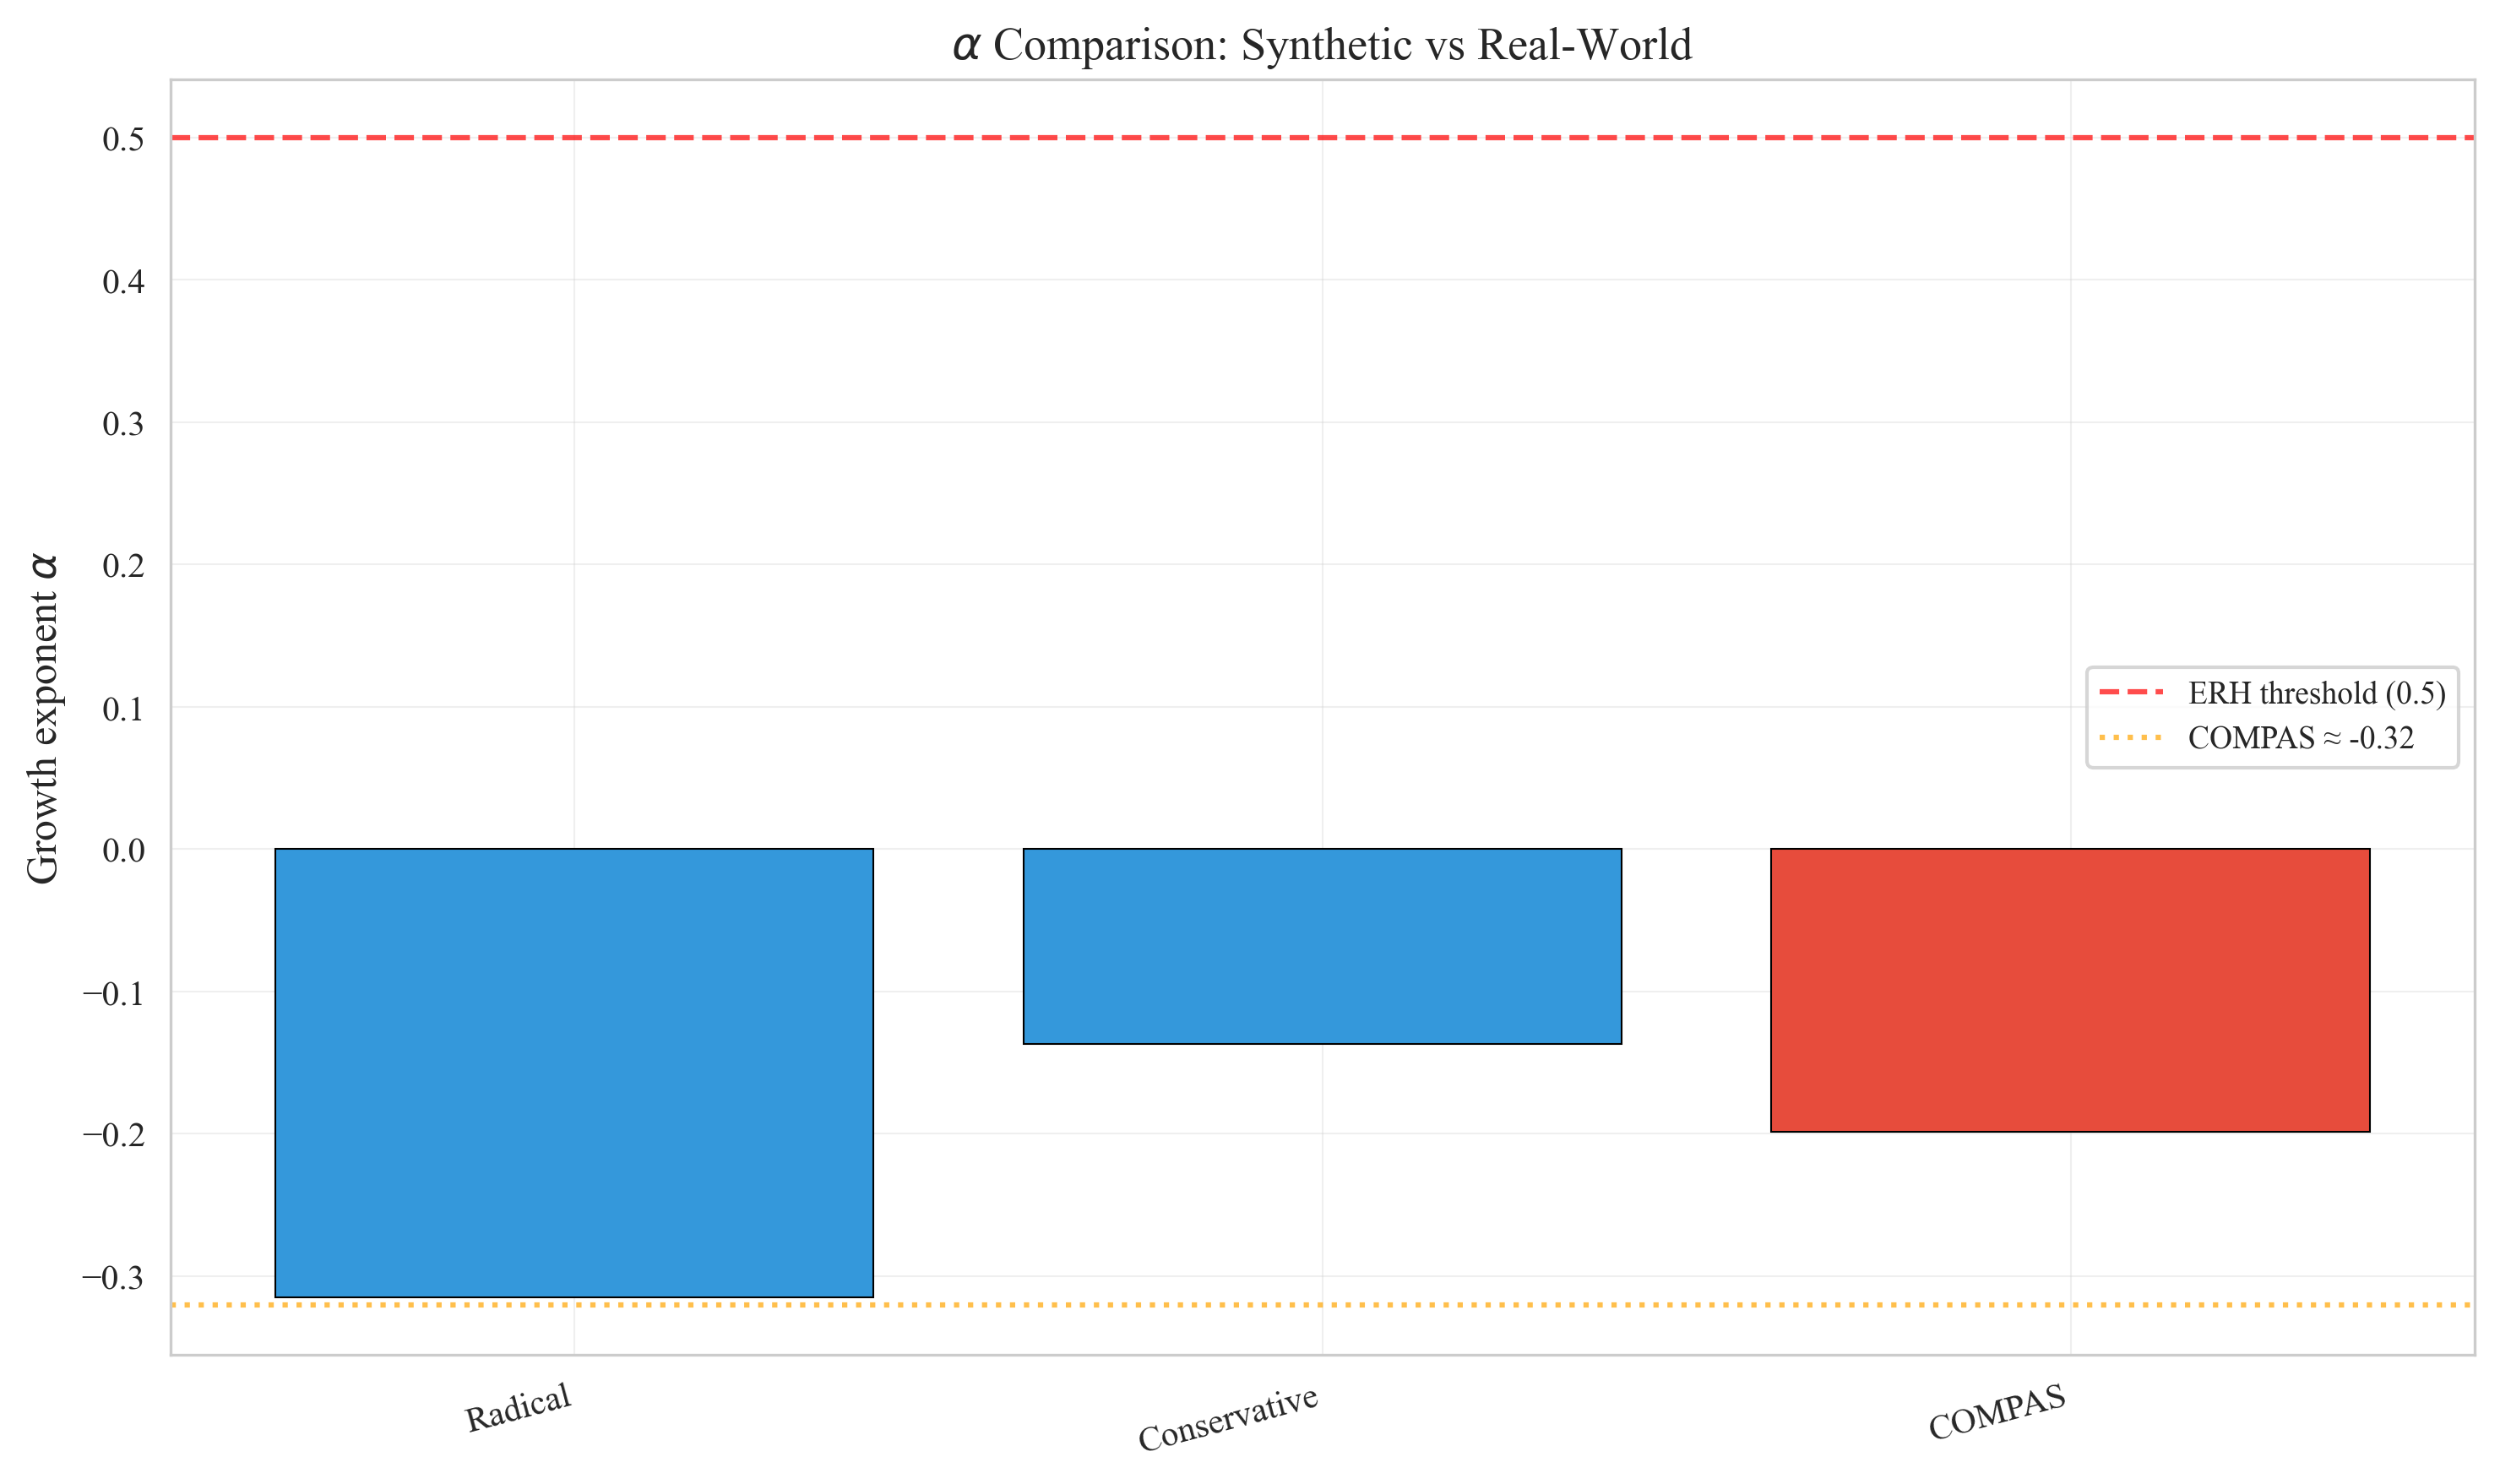
\includegraphics[width=0.8\textwidth]{../simulation/output/figures/alpha_comparison_bar.png}
    }{
      \missingfigureplaceholder
    }
  }
  \caption{Radical、Conservative（模擬）、COMPAS 與 Adult Income 案例研究之擬合增長指數比較。特別標示 COMPAS $\approx-0.20$，以對照真實資料結果與模擬基線。}
  \label{fig:alpha_comparison_bar}
\end{figure}




\subsection{補充流程圖表}

建構流程（\texttt{build\_thesis\_gated.yml}）除了主論文圖表外，還會產生額外的補充圖表。這些圖表由模擬工作流程（真實資料與模擬 $\alpha$ 的比較、含錯誤率與倫理可行性分數的綜合報告）以及當 API 金鑰可用時的 LLM 壓力測試所產生。它們補充核心結果，提供跨複雜度分布（zipf、uniform、power-law）的活動級彙總、與 Adult Income 及 COMPAS 資料集的真實世界驗證，以及來自 LLM 道德判斷的實證 $\Pi(x)$ / $E(x)$ 曲線。若可用，將整合於下方最終 PDF。
% 補充流程圖表將由 integrate_figures.py 插入此處

\begin{figure}[htbp]
  \centering
  \IfFileExists{../figures/normalized_error_oscillation.png}{
    
\includegraphics[width=0.8\textwidth]{../figures/normalized_error_oscillation.png}
  }{
    \IfFileExists{../simulation/output/figures/normalized_error_oscillation.png}{
      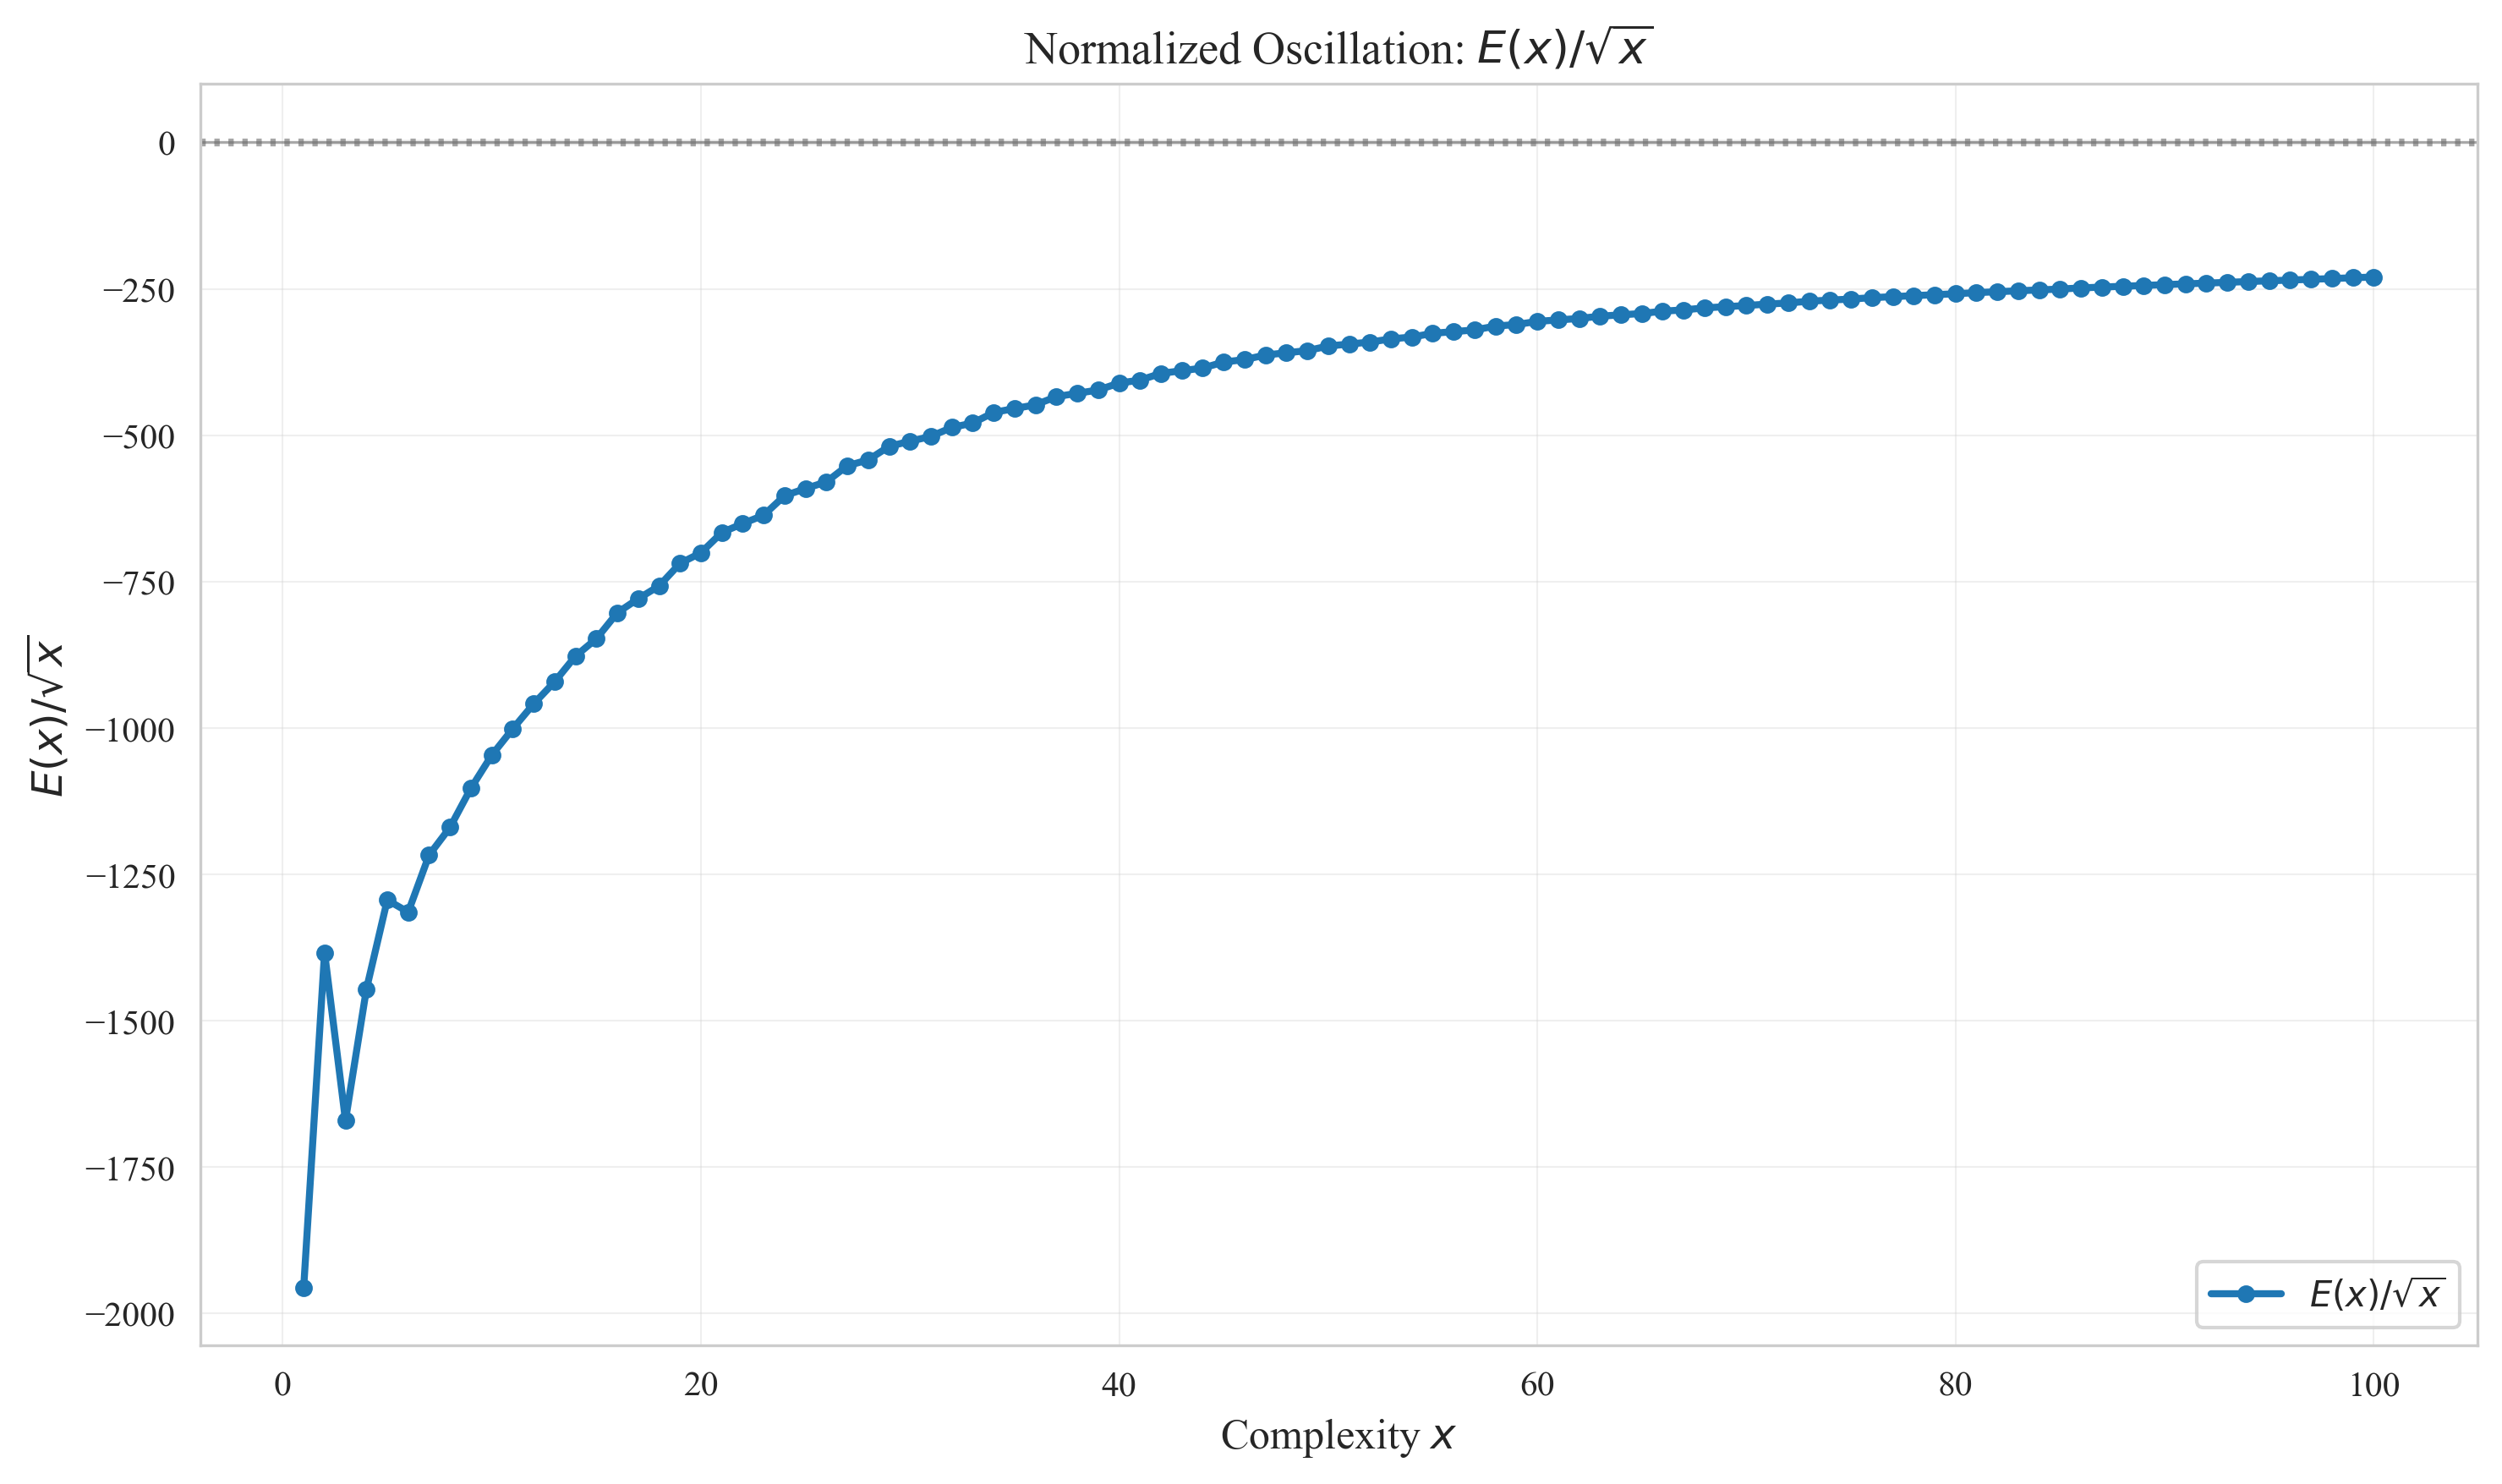
\includegraphics[width=0.8\textwidth]{../simulation/output/figures/normalized_error_oscillation.png}
    }{
      \missingfigureplaceholder
    }
  }
  \caption{COMPAS 的正規化誤差振盪 $E(x)/\sqrt{x}$ 與信賴區間。可用於檢查 ERH 式正規化下是否保持有界，但不應視為公平性指標。}
  \label{fig:normalized_oscillation_compas_zh}
\end{figure}

\begin{figure}[htbp]
  \centering
  \IfFileExists{../figures/latest_quantum_circuit.png}{
    \includegraphics[width=0.8\textwidth]{../figures/latest_quantum_circuit.png}
  }{
    \IfFileExists{../simulation/output/figures/latest_quantum_circuit.png}{
      \includegraphics[width=0.8\textwidth]{../simulation/output/figures/latest_quantum_circuit.png}
    }{
      \missingfigureplaceholder
    }
  }
  \caption{代表倫理 Hilbert 空間的量子電路：$U3$ 門編碼 Bloch 球面位置，$R_{ZZ}$ 門模型社會糾纏。}
  \label{fig:quantum_circuit_supp}
\end{figure}

\begin{figure}[htbp]
  \centering
  \IfFileExists{../figures/latest_quantum_distribution.png}{
    
\includegraphics[width=0.8\textwidth]{../figures/latest_quantum_distribution.png}
  }{
    \IfFileExists{../simulation/output/figures/latest_quantum_distribution.png}{
      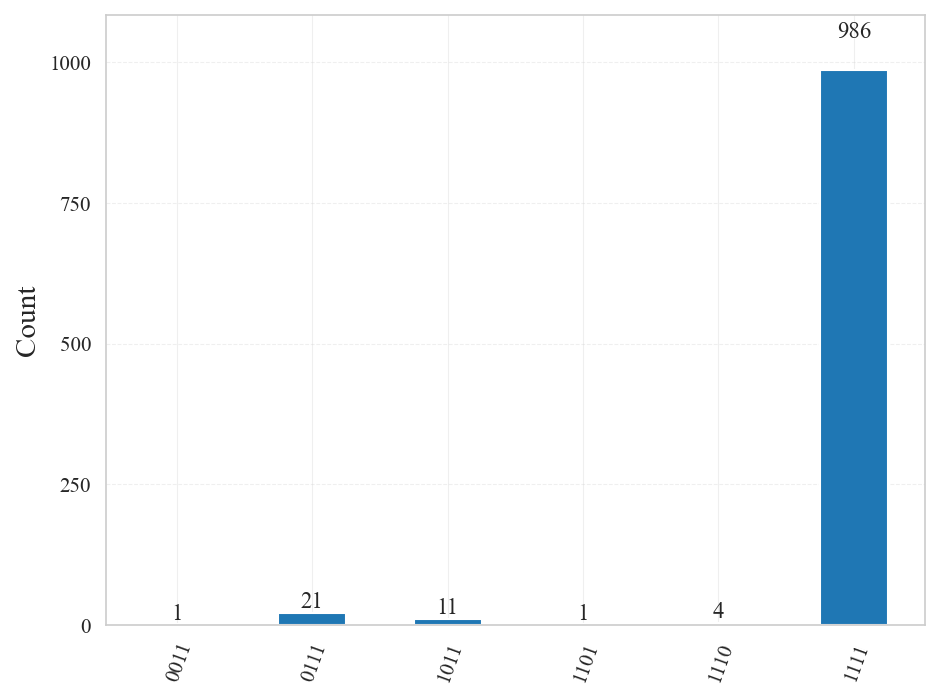
\includegraphics[width=0.8\textwidth]{../simulation/output/figures/latest_quantum_distribution.png}
    }{
      \missingfigureplaceholder
    }
  }
  \caption{量子模擬後倫理態的機率分布。峰值表示高機率社會配置。}
  \label{fig:quantum_dist_supp}
\end{figure}




% ============================================
% 第八節：20 個模擬案例與進階監控
% ============================================
\section{實證驗證：20 個模擬案例}
\label{sec:20_cases}

為了驗證 ERH 框架在不同高風險領域的普適性，我們模擬了 20 個對應現實 AI 應用的具體場景。這些案例涵蓋了司法與安全、醫療倫理、金融與分配、人力資源、數位治理、教育及新興風險（LLM）。

\begin{table}[htbp]
\centering
\caption{20 個模擬案例的彙整結果。錯誤率、倫理質數數量與 $\alpha$ 為各類別的平均值；ERH 通過率表示該類別中被模擬管線標記為 ERH satisfied 的案例比例。}
\label{tab:20_cases_summary_zh}
\begin{tabular}{lcccc}
\toprule
\textbf{類別} & \textbf{錯誤率} & \textbf{質數數量} & \textbf{$\alpha$} & \textbf{ERH 通過率} \\
\midrule
司法與安全     & 0.529 & 6.0 & $0.542$ & 100\% \\
醫療倫理       & 0.362 & 5.0 & $0.714$ & 66.7\% \\
金融與分配     & 0.386 & 3.7 & $0.549$ & 100\% \\
人力資源       & 0.572 & 6.5 & $0.560$ & 100\% \\
數位治理       & 0.482 & 5.3 & $0.556$ & 100\% \\
教育學術       & 0.477 & 5.0 & $0.506$ & 100\% \\
新興風險 (LLM) & 0.444 & 5.5 & $0.548$ & 100\% \\
\bottomrule
\end{tabular}
\end{table}

模擬結果顯示，不同領域的絕對錯誤率差異明顯，而類別平均 $\alpha$ 多半落在 ERH 臨界區附近。若依模擬管線的案例級 ERH 標記統計，除醫療倫理類別因 Organ Matching 個案而降為 66.7\% 外，其餘類別皆為 100\% 通過率；因此此節更適合解讀為「大多數案例維持結構穩定，但仍存在明確離群案例」，而非宣稱所有平均 $\alpha$ 都低於 0.5。

\subsection{20 個模擬案例詳細分析}

以下提供所有 20 個模擬場景的詳細性能指標，按領域分類。

\subsubsection{司法與安全}

\textbf{假釋申請預測 (Parole Board)}：分析假釋申請的預測穩健性。
\begin{itemize}
    \item 錯誤率：0.377
    \item 倫理質數數量：5
    \item 估計指數 ($\alpha$)：$0.520$
    \item ERH 滿足：是
\end{itemize}

\textbf{恐怖主義風險評估 (Terrorism Screening)}：針對安全領域的高風險評估。
\begin{itemize}
    \item 錯誤率：0.658
    \item 倫理質數數量：9
    \item 估計指數 ($\alpha$)：$0.570$
    \item ERH 滿足：是
\end{itemize}

\textbf{兒福預警系統 (CPS)}：兒童保護服務中的風險建模。
\begin{itemize}
    \item 錯誤率：0.551
    \item 倫理質數數量：4
    \item 估計指數 ($\alpha$)：$0.536$
    \item ERH 滿足：是
\end{itemize}

\subsubsection{醫療倫理}

\textbf{急診室檢傷分類 (ER Triage)}：急診室病患優先級排序。
\begin{itemize}
    \item 錯誤率：0.409
    \item 倫理質數數量：6
    \item 估計指數 ($\alpha$)：$0.493$
    \item ERH 滿足：是
\end{itemize}

\textbf{器官移植排序 (Organ Matching)}：移植系統中的資源分配。
\begin{itemize}
    \item 錯誤率：0.067
    \item 倫理質數數量：6
    \item 估計指數 ($\alpha$)：$1.074$
    \item ERH 滿足：否
\end{itemize}

\textbf{精神健康危機介入 (Mental Health Crisis)}：精神科急診的自動化介入。
\begin{itemize}
    \item 錯誤率：0.610
    \item 倫理質數數量：3
    \item 估計指數 ($\alpha$)：$0.575$
    \item ERH 滿足：是
\end{itemize}

\subsubsection{金融與分配}

\textbf{微小型貸款審核 (Micro-finance)}：針對無信用記錄者的貸款審核。
\begin{itemize}
    \item 錯誤率：0.486
    \item 倫理質數數量：5
    \item 估計指數 ($\alpha$)：$0.503$
    \item ERH 滿足：是
\end{itemize}

\textbf{保險費率動態定價 (Insurance Pricing)}：基於複雜行為的動態保費。
\begin{itemize}
    \item 錯誤率：0.251
    \item 倫理質數數量：2
    \item 估計指數 ($\alpha$)：$0.600$
    \item ERH 滿足：是
\end{itemize}

\textbf{社會福利資格自動審核 (Welfare Eligibility)}：社會保障分配的自動化。
\begin{itemize}
    \item 錯誤率：0.420
    \item 倫理質數數量：4
    \item 估計指數 ($\alpha$)：$0.545$
    \item ERH 滿足：是
\end{itemize}

\subsubsection{職場與人力資源}

\textbf{簡歷篩選 (Resume Screening)}：跨領域人才的自動化過濾。
\begin{itemize}
    \item 錯誤率：0.725
    \item 倫理質數數量：8
    \item 估計指數 ($\alpha$)：$0.590$
    \item ERH 滿足：是
\end{itemize}

\textbf{績效考核 AI (Performance Evaluation)}：在高壓環境下的貢獻分析。
\begin{itemize}
    \item 錯誤率：0.418
    \item 倫理質數數量：5
    \item 估計指數 ($\alpha$)：$0.529$
    \item ERH 滿足：是
\end{itemize}

\subsubsection{數位治理與基礎設施}

\textbf{仇恨言論審核 (Hate Speech)}：針對語言複雜或具諷刺性內容的審核。
\begin{itemize}
    \item 錯誤率：0.658
    \item 倫理質數數量：8
    \item 估計指數 ($\alpha$)：$0.585$
    \item ERH 滿足：是
\end{itemize}

\textbf{智慧電網負載平衡 (Smart Grid)}：極端天氣條件下的資源分配。
\begin{itemize}
    \item 錯誤率：0.256
    \item 倫理質數數量：5
    \item 估計指數 ($\alpha$)：$0.522$
    \item ERH 滿足：是
\end{itemize}

\textbf{難民身份認定支援系統 (Refugee Status)}：處理複雜的移民與地緣風險歷史。
\begin{itemize}
    \item 錯誤率：0.533
    \item 倫理質數數量：3
    \item 估計指數 ($\alpha$)：$0.562$
    \item ERH 滿足：是
\end{itemize}

\subsubsection{教育與學術}

\textbf{大學入學多元評價 (Admission Evaluation)}：評估非典型的學生經歷。
\begin{itemize}
    \item 錯誤率：0.486
    \item 倫理質數數量：5
    \item 估計指數 ($\alpha$)：$0.503$
    \item ERH 滿足：是
\end{itemize}

\textbf{自動化論文評分系統 (AES Essay Scoring)}：針對創意性與非標準寫作的評分。
\begin{itemize}
    \item 錯誤率：0.467
    \item 倫理質數數量：5
    \item 估計指數 ($\alpha$)：$0.510$
    \item ERH 滿足：是
\end{itemize}

\subsubsection{新興風險 (LLM)}

\textbf{代碼漏洞掃描 (Code Vulnerability SAST)}：掃描複雜邏輯中的安全性漏洞。
\begin{itemize}
    \item 錯誤率：0.292
    \item 倫理質數數量：4
    \item 估計指數 ($\alpha$)：$0.560$
    \item ERH 滿足：是
\end{itemize}

\textbf{版權合規性檢測 (Copyright Compliance)}：評估高混合度創意作品中的侵權風險。
\begin{itemize}
    \item 錯誤率：0.381
    \item 倫理質數數量：10
    \item 估計指數 ($\alpha$)：$0.548$
    \item ERH 滿足：是
\end{itemize}

\textbf{虛假訊息檢測 (Fake News Detection)}：識別合成媒體中的虛假訊息。
\begin{itemize}
    \item 錯誤率：0.551
    \item 倫理質數數量：3
    \item 估計指數 ($\alpha$)：$0.575$
    \item ERH 滿足：是
\end{itemize}

\textbf{邊緣運算決策 (Edge AI Decision)}：高雜訊環境下的實時決策。
\begin{itemize}
    \item 錯誤率：0.552
    \item 倫理質數數量：5
    \item 估計指數 ($\alpha$)：$0.510$
    \item ERH 滿足：是
\end{itemize}

\subsection{進階倫理監控與代數精確化}

除了啟發式的審計，我們還實現了以下進階功能，將 ERH 從理論分析推向形式化結構監控：

\begin{itemize}
    \item \textbf{代數精確化（奇點定義）}：將倫理質數定義為道德流形上的「奇點」，即誤差地景的拉普拉斯算子（曲率）超過閾值的點。實測流形粗糙度（Roughness）為 0.1349。
    \item \textbf{對抗性倫理質數}：利用模擬退火算法，識別能誘發結構性不穩定的針對性複雜度擾動，為系統提供「紅隊測試」基準。
    \item \textbf{動態 ERH（倫理漂移）}：開發了實時監控器追蹤 $\alpha$ 隨時間的偏移。在模擬的衰減場景中，當 $\alpha$ 漂移至 $-0.255$ 時，監控器成功發出「CRITICAL（關鍵）」警告。
    \item \textbf{多維倫理 Zeta 函數}：透過將道德價值 $V(a)$ 擴展至向量空間（公平、隱私、安全），計算多維 Zeta 函數 $\zeta_{\mathbf{E}}(s)$，分析不同維度間的零點糾纏。
\end{itemize}

% 20 個案例圖表將由 integrate_figures.py 插入此處

\begin{figure}[htbp]
  \centering
  \IfFileExists{../figures/drift_monitoring.png}{
    \includegraphics[width=0.8\textwidth]{../figures/drift_monitoring.png}
  }{
    \IfFileExists{../simulation/output/figures/drift_monitoring.png}{
      \includegraphics[width=0.8\textwidth]{../simulation/output/figures/drift_monitoring.png}
    }{
      \missingfigureplaceholder
    }
  }
  \caption{實時倫理漂移監控，顯示模擬系統性偏見衰減過程中 alpha 指數隨時間的變化。}
  \label{fig:drift_monitoring}
\end{figure}




\section{哲學意涵}
\label{sec:philosophy}

倫理判斷與質數分布之間的類比引發了深刻的哲學思考。若我們將 ERH 視為結構性要求，實質上是在主張道德進步不僅關乎個別「正確」的決策，更關乎判斷系統本身的長期穩定性。這與美德倫理學（Virtue Ethics）一致，後者強調代理人的特質與一致性，而不僅僅是孤立的行為。

\section{AI 倫理應用}
\label{sec:implications}

\subsection{倫理 AI 的設計標準}

ERH 可作為 AI 判斷系統的\emph{最低限度結構健康要求}：若 $|E(x)|$ 明顯快於 $O(\sqrt{x})$ 增長，表示高複雜度案例中的累積風險可能失控；若系統滿足此界限，則只能說明其長尾誤差沒有爆炸。換言之，ERH 是必要條件，不是充分條件。實務上較穩妥的讀法是將 ERH 與任務指標並讀，而不是把它當成單一的「合格證明」。

\begin{itemize}
    \item \textbf{必要條件}：系統至少不應在複雜案例上出現失控的長尾誤差累積。
    \item \textbf{非充分條件}：即使 $\alpha < 0.5$，系統仍可能有高錯誤率、差校準或嚴重群體不平等。
    \item \textbf{雙重讀法}：ERH 應與準確率、校準、公平性 gap 或領域特定損失一起解讀。
\end{itemize}

\subsection{檢測系統性偏見}

ERH 的明顯違反（例如持續觀察到 $\alpha > 0.5$）表明\emph{系統性失敗模式}：
\begin{itemize}
    \item 近臨界區（$\alpha \approx 0.5$）：高複雜度區域開始接近 ERH 式最壞情況，應提高審查頻率
    \item 違反區（$\alpha > 0.5$）：錯誤累積快於 ERH 式上界，表示長尾風險可能正被放大
    \item 低或負值區（$\alpha \leq 0$）：只代表累積速度受控，不代表系統已公平或可接受
\end{itemize}

此類違反需要調查訓練數據、模型架構或評估協議中的結構性偏見。

\subsection{公平性與問責制}

倫理質數的概念強調\emph{並非所有錯誤都是相等的}。對邊緣化群體的高重要性誤判可能在聚合指標中代表性不足，但在倫理質數集合中占主導地位。

基於 ERH 的分析可以：
\begin{itemize}
    \item 識別哪些子群體遭受關鍵誤判
    \item 量化錯誤模式是否在不同人口統計群體之間不同
    \item 指出哪些地方值得進一步做有針對性的干預與傷害分析
\end{itemize}

\subsection{實際應用}

較可信的近期路線包括：
\begin{itemize}
    \item \textbf{高風險排序系統審計}：例如累犯預測或資源分配模型，檢查高複雜度個案是否累積過多關鍵誤判
    \item \textbf{緩解策略比較}：在同一任務上比較不同訓練或重加權方案，觀察其是否同時改善任務指標與 ERH 型態
    \item \textbf{持續監測儀表板}：把 $\alpha$ 或正規化振盪當成輔助警訊，而不是單獨的部署門檻
\end{itemize}

為了支援上述應用，本研究所使用的模擬腳本、設定檔、詳細日誌與生成報告皆已公開於 \url{https://github.com/dennislee928/Ethic-Latex}，其中彙整實驗結果的 \texttt{docs/EXPERIMENT\_REPORTS.md} 與 \texttt{simulation/output/} 目錄可作為主要的補充材料來源。

% ============================================
% 第九節：結論
% ============================================
\section{結論與未來工作}
\label{sec:conclusion}

\subsection{貢獻總結}

本文介紹了倫理黎曼猜想（ERH），這是一個透過與質數理論的類比來分析道德判斷錯誤的數學框架。我們的主要貢獻包括：

\begin{enumerate}
    \item \textbf{數學形式化}：建立了倫理質數及其分布的嚴謹數學框架，定義了行動空間、判斷系統、誤差項與基準函數，並提供了不同判斷者類型的理論區分。
    \item \textbf{ERH 標準}：提出了健康判斷系統的定量標準 $|E(x)| = O(x^{1/2+\varepsilon})$，作為評估系統結構性健康的必要約束。
    \item \textbf{計算工具}：開發了完整的模擬框架與實證測試工具，包含可重現的實驗設計與詳細的統計分析。
    \item \textbf{實證發現}：透過四種判斷策略的比較實驗，證明不同系統表現出顯著不同的錯誤模式，且誤差增長模式優於 ERH 預測並不能保證整體判斷品質。
    \item \textbf{哲學整合}：建立了 ERH 與結果主義、義務論、美德倫理學等古典道德理論的聯繫，並討論了其在不同應用情境下的定位與限制。
    \item \textbf{實際應用}：為 AI 倫理系統的審計、比較與改進提供了定量診斷工具與優先排序機制。
\end{enumerate}

此框架引入了一種透過結構穩定性來審視 AI 道德可靠性的視角。正如心電圖（ECG）監控心律的規律性，以便在心臟驟停發生前偵測到潛在病理，ERH 式診斷則監控累積錯誤在不同複雜度級別間的「律動」，以便在災難性失敗蔓延前標記結構性不穩定。對於政策制定者和審計者而言，這提供了一個關鍵的早期預警系統，與傳統的準確率快照相輔相成。

這項工作開闢了 AI 倫理的新方向：透過解析數論的透鏡來分析道德判斷的結構性模式。雖然與質數的類比是啟發性的而非精確的，但它為評估大規模判斷系統提供了有價值的直覺、定量工具與診斷框架。

\subsection{未來工作}

基於本研究的發現與研究藍圖，我們確定了幾個高優先級的擴展方向：

\begin{itemize}
    \item \textbf{定義的代數化精確}：利用代數幾何或拓撲學，將「倫理質數」定義為道德流形（Moral Manifold）上的奇點，從目前的啟發式篩選轉向嚴謹的結構定義。
    \item \textbf{ERH 正則化與事前約束}：將 ERH 指標直接寫入機器學習的損失函數（Loss Function），在訓練過程中懲罰那些在高複雜度下誤差增長過快的梯度方向。
    \item \textbf{對抗性倫理質數}：研究人為誘發的倫理質數，測試系統在面臨惡意誤導或針對性複雜度擾動時的「結構性防禦能力」。
    \item \textbf{動態 ERH 與生命週期監控}：開發實時監控工具，通過追蹤 $\alpha$ 指數的偏移來檢測系統運行過程中的「倫理漂移（Ethical Drift）」。
    \item \textbf{多維倫理 Zeta 函數}：考慮公平性、隱私性、安全性等多個維度，定義複數空間中的向量 Zeta 函數，分析不同倫理準則之間是否存在「零點糾纏」。
    \item \textbf{社會系統的能譜分析}：引入隨機矩陣理論，利用社會共識系統的能階分布來預測道德相變的臨界點與群體共識的穩定性。
    \item \textbf{人機協作下的 ERH}：模擬「人機共同決策」系統的 ERH 表現，測試人類介入是否能有效地壓低系統的結構性誤差增長。
    \item \textbf{實證案例拓展}：優先在司法預警（假釋、兒福）、醫療倫理（分級診療、資源分配）、金融風控與數位治理等高風險領域進行更大規模的驗證。
\end{itemize}

\subsection{開放問題與反思}

本研究引發了幾個深層次的開放問題：

首先，\emph{我們能否設計出滿足 ERH 的 AI 系統？}我們的實驗結果顯示，即使是「不健康」的系統（如高錯誤率的保守判斷者）也可能在誤差增長模式上優於 ERH 預測，這提醒我們 ERH 提供的是必要而非充分條件。若無法設計出同時滿足 ERH 且具有低整體錯誤率的系統，這是否揭示了自動化道德推理的固有限制？

其次，\emph{道德判斷系統「結構性健康」的真正意涵是什麼？}ERH 提供了一個基於誤差增長模式的答案，但在多元化的道德價值觀與文化背景下，這個定義本身可能受到質疑。不同哲學立場（結果主義、義務論、美德倫理學）可能對「健康」有不同的理解，ERH 框架如何在這種多元性中提供共同的分析語言？

最後，\emph{ERH 框架在實際 AI 倫理決策中的角色定位為何？}是作為診斷工具、隱喻框架，還是有限度的設計約束？我們的哲學分析表明，答案可能因應用情境而異：在標準化決策環境中，ERH 最適合作為最低結構要求與審計訊號；在價值多元化的情境中，它主要作為啟發式分析框架。

這些開放問題不僅指向未來研究的具體方向，更反映了 AI 倫理這一跨學科領域的複雜性與挑戰。

\section*{致謝}

本研究感謝所有為本文提供寶貴建議與反饋的同行。特別感謝 胡君毅先生 在研究過程中提供的指導與支持。本研究使用的開源軟體工具與 Python 生態系統為實驗分析提供了重要基礎。所有模擬程式碼與實驗數據均已公開至https://github.com/dennislee928/Ethic-Latex，以便於研究社群的重現與進一步發展。

\bibliographystyle{plainnat}
\bibliography{references}

\end{document}
